\documentclass[9pt, hyperref={pdfusetitle,colorlinks=true,allcolors=DarkBlue}]{beamer}

% Note: theorems broken when ending with equation, add \vspace{-2ex} to fix.
\usetheme[
    numbering=fraction,
    progressbar=head,
    sectionpage=simple,
    block=fill,
]{metropolis}

% Include packages and definitions
\usepackage{packages}
% Define custom colors
\definecolor{DarkBlue}{HTML}{36587E}
\definecolor{DarkGreen}{HTML}{006600}
\definecolor{BrightOrange}{HTML}{EB811B}

% Define matplotlib color
\definecolor{C1}{HTML}{1f77b4}
\definecolor{C2}{HTML}{ff7f0e}
\definecolor{C3}{HTML}{2ca02c}
\definecolor{C4}{HTML}{d62728}
\definecolor{C5}{HTML}{9467bd}
\definecolor{C6}{HTML}{8c564b}
\definecolor{C7}{HTML}{e377c2}
\definecolor{C8}{HTML}{7f7f7f}
\definecolor{C9}{HTML}{bcbd22}
\definecolor{C10}{HTML}{17becf}

% PDF encoding
\def\texpdf#1#2{\texorpdfstring{#1}{#2}}

% Figures
\def\imagebox#1#2{\vtop to #1{\null\hbox{#2}\vfill}}

% Text locutions
\def\ie{i.e.\@}
\def\eg{e.g.\@}
\def\resp{resp.\@}
\def\wrt{w.r.t.\@}

% Overwrite commands
\def\epsilon{\varepsilon}

% Backslash capital case for calligraphic
\def\A{\mathcal A}
\def\B{\mathcal B}
\def\C{\mathcal C}
\def\D{\mathcal D}
\def\E{\mathcal E}
\def\F{\mathcal F}
\def\G{\mathcal G}
\def\H{\mathcal H}
\def\I{\mathcal I}
\def\J{\mathcal J}
\def\K{\mathcal K}
\def\L{\mathcal L}
\def\M{\mathcal M}
\def\N{\mathcal N}
\def\O{\mathcal O}
\def\P{\mathcal P}
\def\Q{\mathcal Q}
\def\R{\mathcal R}
\def\S{\mathcal S}
\def\T{\mathcal T}
\def\U{\mathcal U}
\def\V{\mathcal V}
\def\W{\mathcal W}
\def\X{\mathcal X}
\def\Y{\mathcal Y}
\def\Z{\mathcal Z}

% Backslash lower case for bold
\def\a{\mathbf a}
\def\b{\mathbf b}
\def\c{\mathbf c}
\def\d{\mathbf d}
\def\e{\mathbf e}
\def\f{\mathbf f}
\def\g{\mathbf g}
\def\h{\mathbf h}
\def\i{\mathbf i}
\def\j{\mathbf j}
\def\k{\mathbf k}
\def\l{\mathbf l}
\def\m{\mathbf m}
\def\n{\mathbf n}
\def\o{\mathbf o}
\def\p{\mathbf p}
\def\q{\mathbf q}
\def\r{\mathbf r}
\def\s{\mathbf s}
\def\t{\mathbf t}
\def\u{\mathbf u}
\def\v{\mathbf v}
\def\w{\mathbf w}
\def\x{\mathbf x}
\def\y{\mathbf y}
\def\z{\mathbf z}

% Ensemble
\def\NN{\mathbb N}
\def\ZZ{\mathbb Z}
\def\RR{\mathbb R}
\def\CC{\mathds C}

% Special vectors and matrices
\def\0{\mathbf 0}
\def\1{\mathbf 1}
\def\eye{\mathds 1}

% Differential symbol
\def\diff#1{\operatorname{d}\!{#1}}

% Math operators
\DeclareMathOperator*{\expect}{\mathlarger{\mathbb{E}}}
\DeclareMathOperator*{\argmax}{arg\,max}
\DeclareMathOperator*{\argmin}{arg\,min}
\def\sg{\operatorname{sg}}

\newenvironment{psmatrix}{\left(\begin{smallmatrix}}{\end{smallmatrix}\right)}

% Names for autoref command
\def\chapterautorefname{Chapter}
\def\sectionautorefname{Section}
\def\subsectionautorefname{Subsection}
\def\subsubsectionautorefname{Subsubsection}
\def\paragraphautorefname{Paragraph}
\def\tableautorefname{Table}
\def\equationautorefname{Equation}
\def\algorithmautorefname{Algorithm}
\def\figureautorefname{Figure}

% Tikz
\newcommand<>{\uncoverubrace}[2]{%
  \onslide#3 \underbrace{ \onslide<1->%
  #1%
  \onslide#3 }_{#2} \onslide<1->%
}
\newcommand<>{\uncoverobrace}[2]{%
  \onslide#3 \overbrace{ \onslide<1->%
  #1%
  \onslide#3 }^{#2} \onslide<1->%
}



\usepackage{graphicx}
\usepackage{amsmath}
\usepackage{media9}
\usepackage{bm}
\usepackage{dsfont}
\usepackage{ulem}
\usepackage{bm}
\usepackage{url}

\makeatletter
\def\blfootnote{\xdef\@thefnmark{}\@footnotetext}
\makeatother



\author{Pascal Leroy (\href{mailto:pleroy@uliege.be}{pleroy@uliege.be})}
\begin{document}
\title{
INFO8003-1 \\
Optimal decision making for complex problems
\\
\vspace{.7cm}
Multi-Agent Reinforcement Learning
}

\date{April 2024}
\maketitle


\section*{Content}
\begin{frame}{Content}
Today, an overview of multi-agent reinforcement learning (MARL):
\begin{itemize}
\vfill
\item Reinforcement learning basics (SARL)
\vfill
\item Multi-agent reinforcement learning framework
\vfill
\item Cooperative scenarios
\vfill
\item Communication
\vfill
\item Competitive scenarios
\vfill
\item Adversarial attacks
\vfill
\item References
\end{itemize}

\end{frame}

\section{RL basics}


\begin{frame}{RL basics: MDP}
\centering
Single-agent reinforcement learning (SARL)
\vfill 
\begin{columns}
\begin{column}{0.5\textwidth}
Markov decision process (MDP)
    \begin{figure}
    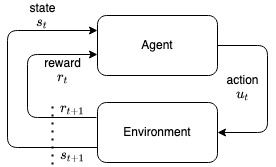
\includegraphics[scale=0.4]{MDP.jpg}
    \caption{RL environment.}
    \end{figure}
\vfill
\end{column}
\begin{column}{0.5\textwidth}  %%<--- here
Defined by:
    \begin{itemize}
        \item A set of states $s \in \mathcal{S}$.
        \item A set of actions \textcolor{red}{$u \in \mathcal{U}$}.
        \item Transition function: $s_{t+1} \sim P(s_{t+1} | s_t, u_t)$.
        \item Reward function: \\ $r_t = R(s_{t+1}, s_t, u_t)$.
        \item Policy: $\pi(u_t|s_t)$.
        % \mathcal{S} \times \mathcal{A} \rightarrow [0, 1]
    \end{itemize}{}
\end{column}
\end{columns}
 
    \vfill
    The agent \textbf{goal} is maximize its total expected sum of discounted rewards $\sum_{t=0}^{T} \gamma^t r_t$ with $\gamma \in [0, 1)$, obtained with the optimal policy $\pi^*$.
    
   \blfootnote{Richard S. Sutton and Andrew G. Barto. 2018. Reinforcement Learning: An Introduction. A Bradford Book, Cambridge, MA, USA.}
\end{frame}



\begin{frame}{RL basics: Value-based methods}
Value-based methods:
\vfill
    \begin{itemize}
    \item State Value of a policy $\pi$:
    \begin{equation*}
    V^\pi(s_t) = \mathbb{E}_\pi \left[r_t + \gamma V^\pi(s_{t+1}) | s_t\right]
    \end{equation*}
    \vfill
    \item State-Action Value of a policy $\pi$:
    \begin{equation*}
    Q^\pi(s_t, u_t)  = \mathbb{E}_\pi \left[r_t + \gamma  Q^\pi(s_{t+1}, u_{t+1}) | s_t, u_t \right]
    \end{equation*}
    \vfill
    \item The optimal policy is:
    \begin{equation*}
    \pi^*(s_t) = \argmax_u Q^{\pi^*}(s_{t}, u)
    \end{equation*}
\end{itemize}{}
\end{frame}

\begin{frame}{RL basics: DQN}
DQN: Q-learning with a neural network parametrised by $\theta$:
\begin{equation*}
    \mathcal{L}(\theta) = \mathds{E}_{\langle s_{t},u_{t},r_{t},s_{t+1}\rangle \sim B} 
    \bigg[  
    \big(r_{t} + \gamma \max_{u \in \mathcal{U}} Q(s_{t+1}, u; \theta')
    - Q(s_{t}, u_{t}; \theta)\big)^{2}\bigg]
    \label{eq:DQN_loss}
\end{equation*}
\vfill
\begin{itemize}
    
    \item The replay buffer $B$ is a collection of transitions.
    \item Sampling transitions allows to update the network.
    \item $\theta'$ denotes the parameters of the \textbf{target network}, a copy of $\theta$ that is periodically updated.
    \vfill
    \item To play Atari games, $\theta$ is a CNN.
    \item When the environment is partially observable (POMDP), $\theta$ is a recurrent network (DRQN) and $B$ stores sequences of transitions.
    
    
\end{itemize}{}
\end{frame}

\begin{frame}{RL basics: Policy-based methods}
\vfill
We denote the discounted sum of reward of a trajectory by 
\begin{equation*}
G_t(\tau)  = \sum_{j=0}^T \gamma^j r_{t+j} \hspace{.5cm} \text{ where } \tau = (s_t, u_t, r_t, s_{t+1}, u_{t+1},.., s_T)
\end{equation*}
\vfill
Reinforce:
\begin{equation*}
        \nabla_\theta J(\theta)  = \mathbb{E}_{\tau \sim \pi_\theta}\left[\left(  \sum_t^T G_t(\tau)  \nabla_\theta  \log \pi_\theta(u_t, s_t)  \right)\right] 
\end{equation*}


\end{frame}

\begin{frame}{RL basics: How to improve reinforce?}

Smaller variance with a baseline $b$:
\begin{equation*}
\nabla_\theta J(\theta)  = \mathbb{E}_{\tau \sim \pi_\theta}\left[ \left( \sum_t^T \left( G_t(\tau)-b \right) \nabla_\theta \log \pi_\theta(a_t, s_t) \right) \right] 
\end{equation*}

\vfill
 
Or Q Actor-Critic:
$$Q(s_t, u_t;\phi) = \mathbb{E}_{(r_t, s_{t+1},...,s_T)}\left[G_t(\tau) \right]$$

$$\nabla_\theta J(\theta)  = \mathbb{E}_{\tau \sim \pi_\theta}\left[\left( \sum_t^T Q(s_t, u_t;\phi) \nabla_\theta  \log \pi_\theta(u_t, s_t) \right) \right] $$




\end{frame}

\begin{frame}{RL basics: Advantage Actor-Critic}

    
Advantage Actor-Critic, the baseline is the Value function:

\begin{itemize}
    \item Actor $\theta$, learns the policy:
    \vfill
    \begin{equation*}
         \nabla_\theta J(\theta)  = \mathbb{E}_{\tau \sim \pi_\theta}\left[ \left(\sum_t^T A(s_t, u_t; \phi) \nabla_\theta \log \pi_\theta(u_t, s_t)  \right) \right] 
    \end{equation*}
    \vfill
    \item Critic $\phi$, learns the advantage $Q(s_t, u_t) - V(s_t)$:
    \vfill
    \begin{equation*}
        A(s_t, u_t; \phi) = r_t + \gamma V(s_{t+1}; \phi) - V(s_t; \phi)
    \end{equation*}
\end{itemize}{}

\end{frame}

\begin{frame}{RL basics: Recap}

    

\begin{itemize}
    \item Markov Decision Process
    \vfill
    \item Value-based methods
        \begin{itemize}
        \item DQN
        \item DRQN
        \end{itemize}{}
    \vfill
    \item Policy-based methods
        \begin{itemize}
        \item Reinforce + improvements
        \item Advantage Actoc-Critic
        \end{itemize}{}
    \vfill
\end{itemize}{}

\end{frame}

\section{Multi-Agent RL}
\begin{frame}{MARL: Framework}
    Stochastic Game (also referred to as Markov Game) $[n, \mathcal{S}, O, \mathcal{Z}, \mathcal{U}, r, P, \gamma]$:
    \vfill
    \begin{itemize}
        \item A set of $n$ agents represented by $a$ or $a_i, i \in  \{1,...,n\}$.
        \vfill
        \item A set of states $s \in \mathcal{S}$.
        \vfill
        \item A set of action spaces $\mathcal{U}=\mathcal{U}_1 \times ... \times \mathcal{U}_n$, one per agent $u^{a_i}_{t} \in \mathcal{U}_i$.
        \vfill
        \item A transition function: $s_{t+1} \sim P(s_{t+1} | s_t, \boldsymbol{u_t})$, $\boldsymbol{u_t}= u^{a_1}_t, ..., u^{a_n}_t$.
        \vfill
        \item A reward function per agent:  $r^{a_i}_t = R^{a_i}(s_{t+1}, s_t, \boldsymbol{u_t})$.
        \vfill
        \item An observation function $O:\mathcal{S} \times \{1,...,n\} \rightarrow \mathcal{Z}$, sometimes defined as a set.
        \vfill
        \item Agents sometimes store their history $\tau^a_t \in (\mathcal{Z} \times \mathcal{U})^t$.
        \vfill
        \item The goal of each agent $a_i$ is to maximize its total expected sum of (discounted) rewards $\sum_{t=0}^{T} \gamma^t r^{a_i}_t$.
    \end{itemize}{}
\end{frame}

\begin{frame}{MARL: Different settings}
In Multi-agent settings, the goal of each agent may differ:
\vfill
\begin{enumerate}
    \item Cooperative setting: all agents share a common goal.
    \\Examples: traffic control, robotics teams,...
    \vfill
    \item Competitive setting: the gain of an agent equals the loss of other agents.
    \\Often referred to as zero-sum setting because all agents' rewards sum to zero.
    \\Examples: board games, video games, GAN,...
    \vfill
    \item General sum setting: lies in between the two others.
    \\Examples: everything that is not cooperative or competitive, 5v5 video games, autonomous vehicles,...
\end{enumerate}
\end{frame}

\section{Cooperative}

\begin{frame}{Cooperative: Dec-POMDP}
In a cooperative setting, it is possible to have a single reward function, each agent receives a same global reward:
\begin{equation*}
    r^{a_1}_t = r^{a_n}_t=r_t = R(s_{t+1}, s_t, \boldsymbol{u_t}): \mathcal{S}^2 \times \mathcal{U} \rightarrow \mathbb{R}
\end{equation*}
Such stochastic Games are called Decentralised-POMDP.
\begin{figure}
    \centering
    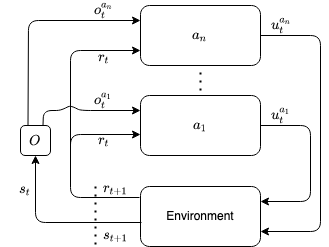
\includegraphics[scale=0.45]{dec-poMDP.png}
    \caption{Dec-POMDP.}

\end{figure}
\end{frame}

\begin{frame}{Cooperative: environment example}
StarCraft multi-agent challenge (SMAC).

Dec-POMDP environment based on StarCraft 2.
 
All agents learn to cooperate against the built-in AI: this is not a competitive setting because the built-in AI is stationary.

\begin{figure}
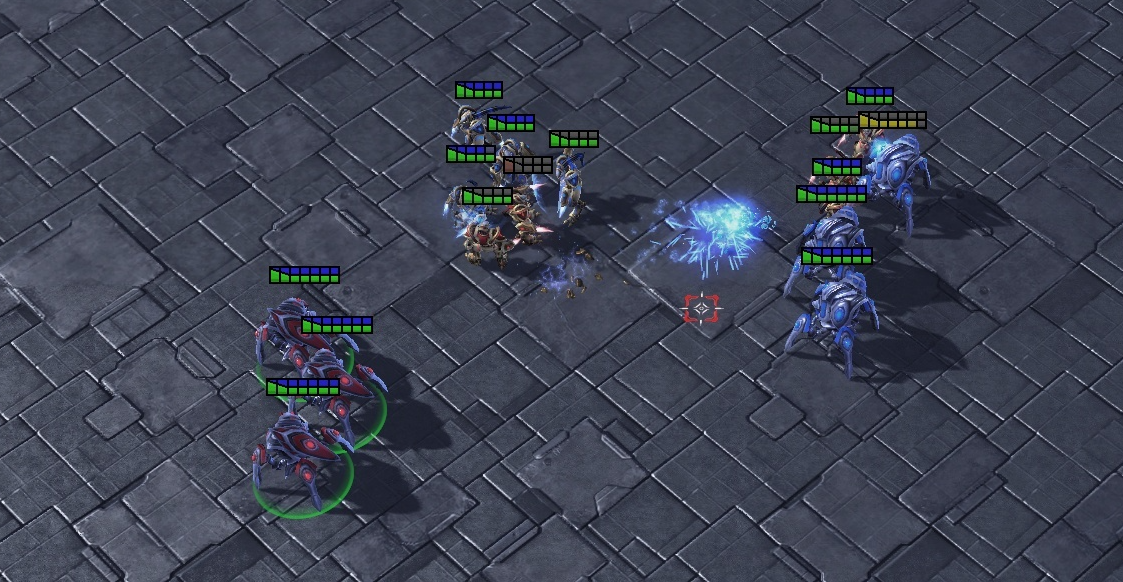
\includegraphics[scale=0.14]{3s5z_sc2.png}
\caption{SMAC example (3s5z).}
\end{figure}
\url{https://github.com/oxwhirl/smac} \url{https://youtu.be/VZ7zmQ_obZ0}

\blfootnote{Samvelyan, M., Rashid, T., De Witt, C. S., Farquhar, G., Nardelli, N., Rudner, T. G., ...  Whiteson, S. (2019). The starcraft multi-agent challenge. }
\end{frame}


\begin{frame}{Cooperative: Centralised controller}
\vfill

Centralised controller:
        \begin{itemize}
            \item One agent controls all actions.
            \item A single joint actions space $\mathcal{U}_1 \times ... \times \mathcal{U}_n$.
        \end{itemize}
    \vfill
Problems?
    \pause
    \begin{itemize}
        \item Joint actions space scales exponentially with $n$.
        \item What about the partial observability?\\
        $\rightarrow$ Not possible to centralise.
    \end{itemize}
    \vfill
Solutions?
    \pause
    \begin{enumerate}
        \item Decentralised controller.\\
        $\rightarrow$ Naive learner: train each agent with SARL methods.
        \item Centralised training with decentralised execution (CTDE).\\
        $\rightarrow$ Benefit from supplementary information during training, such as the entire state of the game.
        \end{enumerate}

\end{frame}

\begin{frame}{Cooperative: Naive learner}
Naive learning:
\begin{itemize}
    \item Ignore the fact that there are multiple learning agents.
    \item Provide a first baseline to compare algorithms.
    \item Easy to implement.
    \item Not so young: a tabular version with IQL (Tan 1993).
\end{itemize}
\vfill
Challenges:
\pause
\begin{itemize}
\item Non-stationarity:

Other agents are also learning and their policy changes over time.

\item Credit assessment: 

How does an agent learn whether their actions are the ones that leads to good (or bad) rewards?

How does an agent maximise the joint actions reward knowing only its action?

\end{itemize}
\end{frame}

\begin{frame}{Cooperative: Value-based methods in CTDE}
Naive learner: Independent Q-Learning (IQL)\\
$\rightarrow$ Each agent learns its individual $Q_a(\tau^a_t, u^a_t)$ independently.
\vfill
Problem:
How to ensure that $\argmax_{u^a_t} Q_a(\tau^a_t, u^a_t)$ maximises $Q(s_t, \bm{u_t})$?
\vfill
\pause
Solution: Learn $Q(s_t, \bm{u_t})$ as a function of all $Q_a(\tau^a_t, u^a_t)$ during training.
\vfill
$Q_a$ are not anymore $Q$ functions but utility functions used to select actions.
\vfill
Condition: Individual Global Max (IGM):
\begin{equation*}
    \argmax_{\bm{u_t}} Q(s_t, \bm{u_t}) = 
    \begin{pmatrix}
    \argmax_{u^{a_1}_t} Q_1(\tau^{a_1}_t, u^{a_1}_t) \\
    : \\
    : \\
    \argmax_{u^{a_n}_t} Q_n(\tau^{a_n}_t, u^{a_n}_t)
    \end{pmatrix}
\end{equation*}

\end{frame}



\begin{frame}{Cooperative: VDN and QMIX}
How to satisfy IGM?

Value Decomposition Network:
\begin{equation*}
    Q(s_t, \bm{u_t}) = \sum_{i=1}^n Q_{a_i}(\tau^{a_i}_t, u^{a_i}_t) 
\end{equation*}
Problems:
\begin{itemize}
    \item Addition does not allow to build complex functions.
    \item Current state information $s_t$ is not considered.
\end{itemize}
\end{frame}

\begin{frame}{Cooperative: QMIX}
How can we build non-linear factorisation satisfying IGM? 
\vfill
QMIX idea is to enforce monotonicity:
\begin{equation*}
    \frac{\partial Q(s_t, \bm{u_t})}{\partial Q_{a}(\tau^{a}_t, u_t^{a})} \geq 0 \text{ } \forall a \in \{a_1,..,a_n\}
\end{equation*}
\vfill
How to build a non-linear monotonic factorisation of $Q(s_t, \bm{u_t})$ as a function of every  $Q_a(\tau^{a}_t, u^a_t)$ and $s_t$ with neural networks?
\vfill
In QMIX, monotonicity is ensured by constraining a hypernetwork that computes the weights of a second neural network.
\end{frame}

\begin{frame}{Cooperative: QMIX architecture}
\begin{figure}
    \centering
    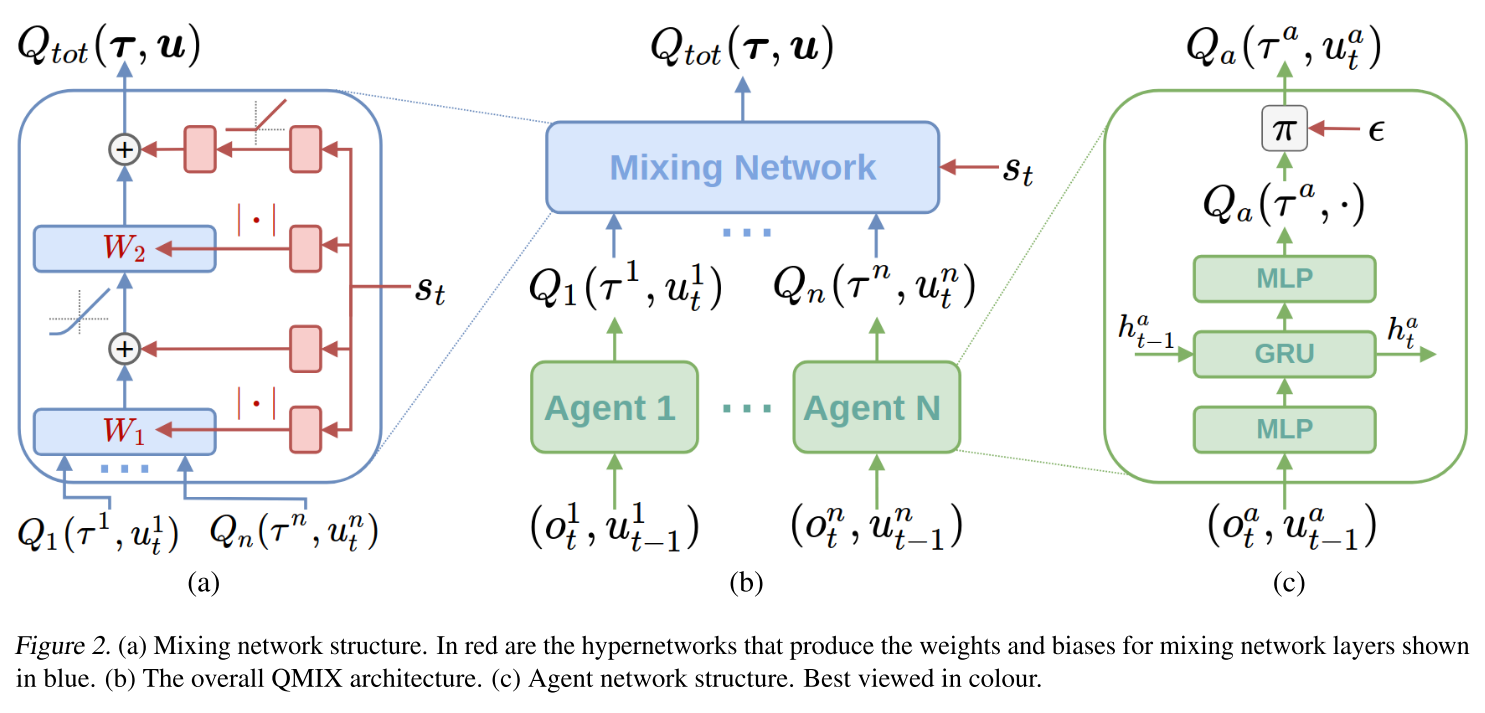
\includegraphics[scale=0.2]{qmix_archi.png}
    \caption{QMIX architecture.}
\end{figure}

\blfootnote{Rashid, T., Samvelyan, M., Schroeder, C., Farquhar, G., Foerster, J., Whiteson, S. (2018). Qmix: Monotonic value function factorisation for deep multi-agent reinforcement learning.}
\end{frame}

\begin{frame}{Cooperative: QMIX}

In QMIX:
\begin{itemize}
    \item \textcolor{red}{A hypernetwork $h_p$} takes the state $s_t$ as input and computes the weights \textcolor{red}{W1} and \textcolor{red}{W2} of a \textcolor{blue}{second neural network}.
    \item \textcolor{red}{These weights} are constrained to be positive and then used in a \textcolor{blue}{feed forward network $h_o$} to factorise $Q(s_t, \bm{u_t})$ with the individual $Q_a$.
    \item A neural network made of monotonic functions and strictly positive weights is monotonic with respect to its inputs.
\end{itemize}

$$\rightarrow Q_{mix}(s_t, \bm{u_t}) = h_o\left(Q_{a_1}(),..,Q_{a_n}(), h_p(s_t)\right)$$

The optimisation procedure follows the same principles of DQN algorithm:
\begin{equation*}
    \mathcal{L}(\theta) = \mathds{E}_{\langle . \rangle \sim B} 
    \bigg[  
    \big(r_{t} + \gamma \max_{\bm{u} \in \mathcal{U}} Q_{mix}(s_{t+1}, \bm{u}; \theta')
    - Q_{mix}(s_{t}, \bm{u_{t}}; \theta)\big)^{2}\bigg]
    \label{eq:qmix_loss}
\end{equation*}

Commonly, parameters of individual networks are shared to speed up learning.
\end{frame}



\begin{frame}{Cooperative: QMIX results}
\begin{figure}
    \centering
    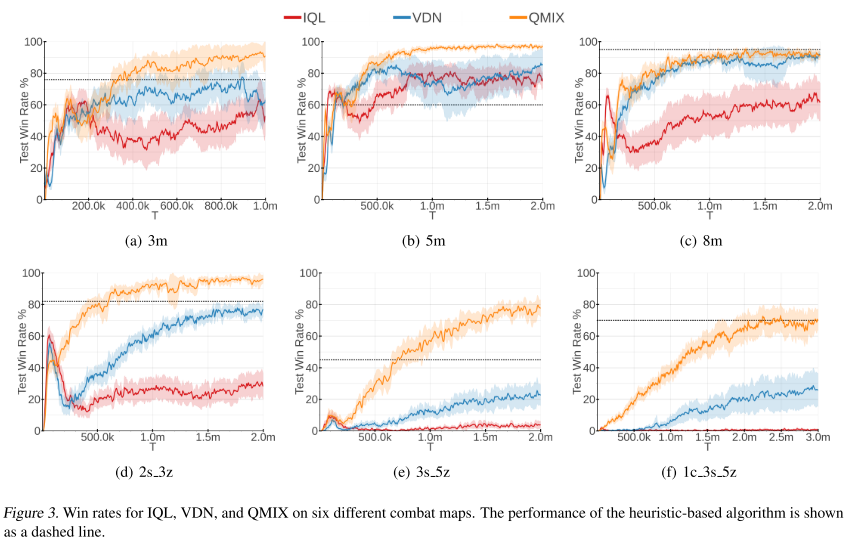
\includegraphics[scale=0.35]{qmix_results.png}
\end{figure}

\blfootnote{Rashid, T., Samvelyan, M., Schroeder, C., Farquhar, G., Foerster, J., Whiteson, S. (2018). Qmix: Monotonic value function factorisation for deep multi-agent reinforcement learning.}
\end{frame}



\begin{frame}{Cooperative: DQV}
Deep-Quality value: learn $Q(.;\theta)$ and $V(.;\phi)$ at the same time.
\begin{equation*}
    \mathcal{L}(\theta) = \mathds{E}_{\langle s_{t},u_{t},r_{t},s_{t+1}
    \rangle\sim B} \bigg[\big(r_{t} + \gamma V(s_{t+1}; \phi') - Q(s_{t}, u_{t}; \theta)\big)^{2}\bigg]
    \label{eq:dqv_q_update}
\end{equation*}
\begin{equation*}
    \mathcal{L}(\phi) = \mathds{E}_{\langle 
    s_{t},u_{t},r_{t},s_{t+1}
    \rangle\sim B} \bigg[\big(r_{t} + \gamma V(s_{t+1}; \phi') - V(s_{t}; \phi)\big)^{2}\bigg]
    \label{eq:dqv_v_update}
\end{equation*}
\vfill
Benefit of DQV is to reduce the overestimation problem of DQN, linked to the max operator.

DQN loss reminder:
\begin{equation*}
    \mathcal{L}(\theta) = \mathds{E}_{\langle s_{t},u_{t},r_{t},s_{t+1}\rangle \sim B} 
    \bigg[  
    \big(r_{t} + \gamma \max_{u \in \mathcal{U}} Q(s_{t+1}, u; \theta')
    - Q(s_{t}, u_{t}; \theta)\big)^{2}\bigg]
    \label{eq:DQN_loss_2}
\end{equation*}
\end{frame}

\begin{frame}{Cooperative: QVMix}
QVMix and QVMix-Max are extensions of the Deep-Quality value family of algorithms to cooperative multi-agent.
\vfill
QVMix:
\begin{equation}
    \mathcal{L}(\theta) = \mathds{E}_{\langle .
    \rangle\sim B} \bigg[\big(r_{t} + \gamma V(s_{t+1}; \phi') - Q(s_{t}, \bm{u_{t}}; \theta)\big)^{2}\bigg]
    \label{eq:dqv_qvmix_q_update}
\end{equation}
\begin{equation}
    \mathcal{L}(\phi) = \mathds{E}_{\langle 
    .
    \rangle\sim B} \bigg[\big(r_{t} + \gamma V(s_{t+1}; \phi') - V(s_{t}; \phi)\big)^{2}\bigg]
    \label{eq:dqv_qvmix_v_update}
\end{equation}
\vfill
QVMix-Max:
\vfill
\begin{equation}
    \mathcal{L}(\phi) = \mathds{E}_{\langle 
    .
    \rangle\sim B} \bigg[\big(r_{t} + \gamma \max_{\bm{u} \in \mathcal{U}} Q(s_{t+1}, \bm{u}; \theta') - V(s_{t}; \phi)\big)^{2}\bigg]
    \label{eq:dqv_qvmix_max_update}
\end{equation}
\vfill
In QVMix, the architecture of $V$ and $Q$ are the same as $Q$ in QMIX, except for $V$ that has a single output since actions are ignored.
\end{frame}

\begin{frame}{Cooperative: QVMix results}
\begin{figure}
    \centering
    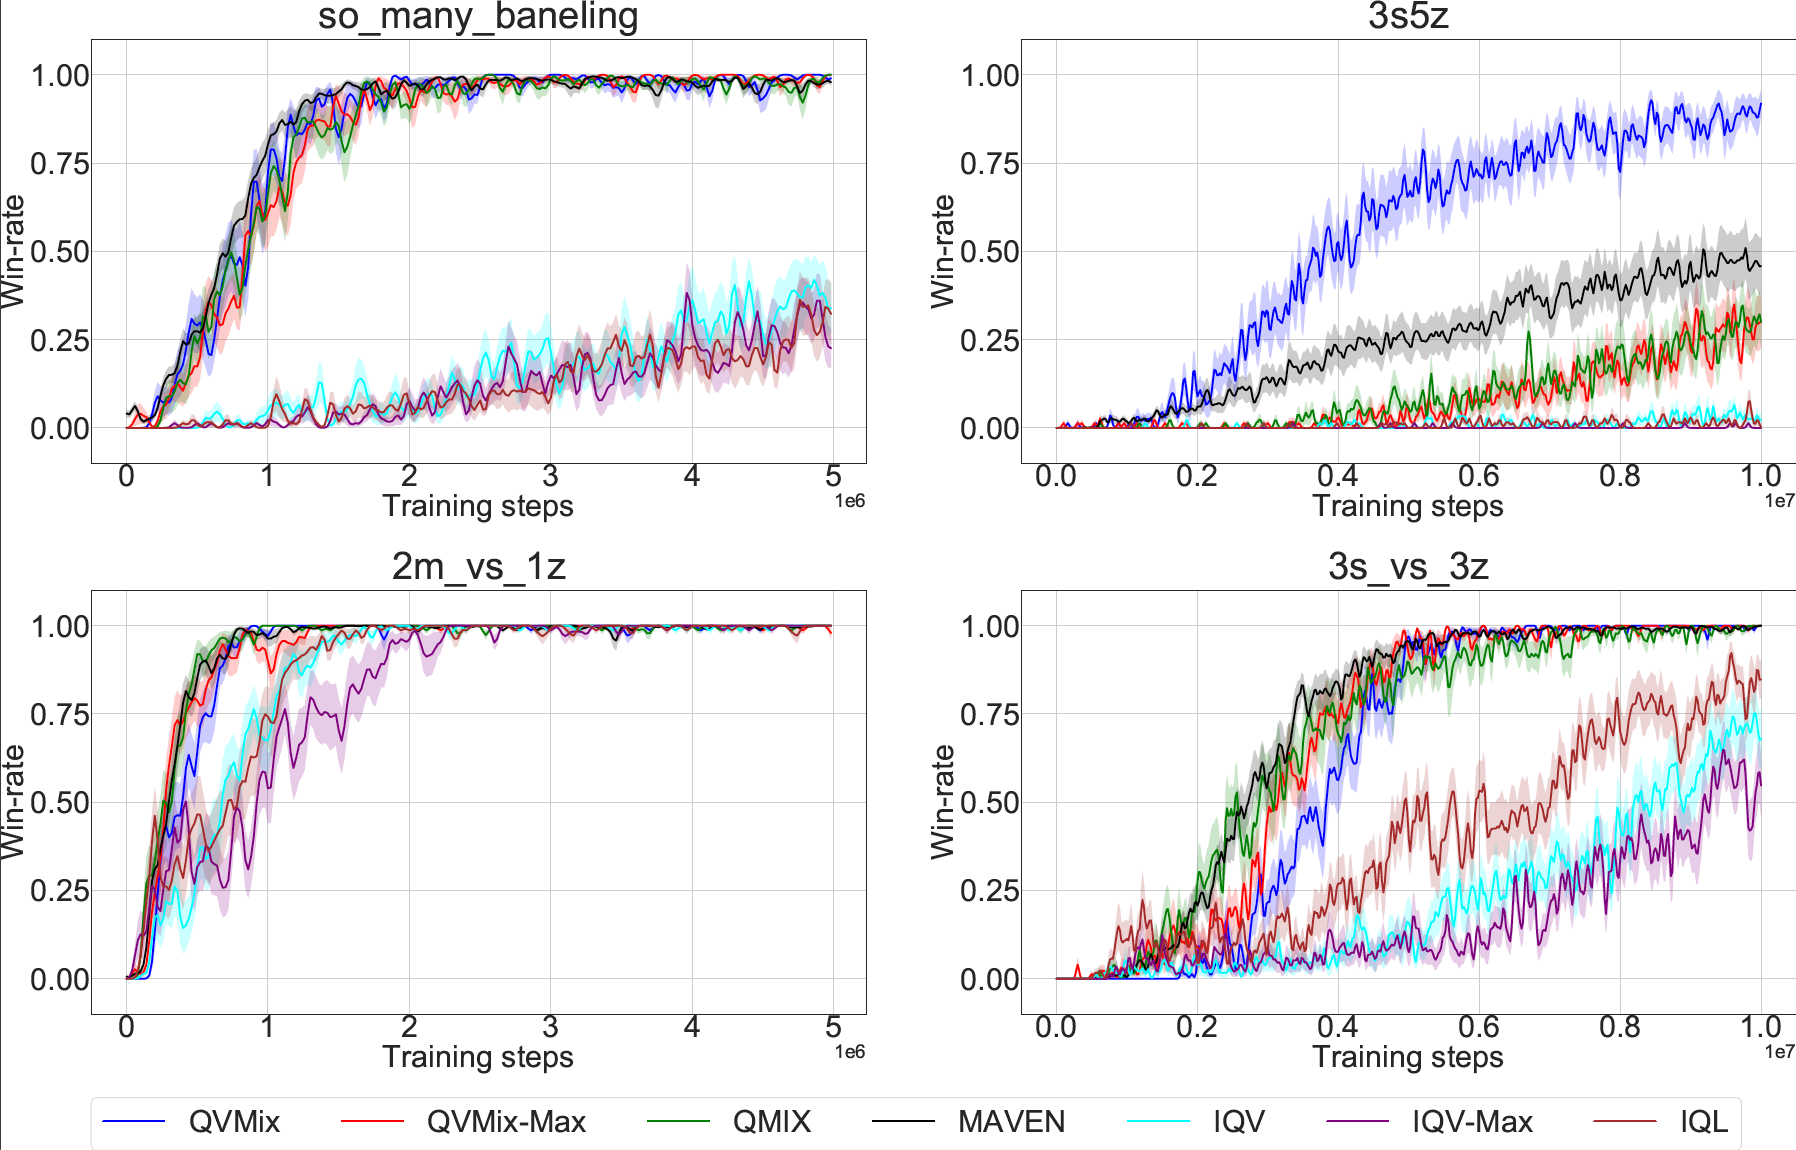
\includegraphics[width=\textwidth]{qvmix_results.png}
\end{figure}
\blfootnote{Leroy, P., Ernst, D., Geurts, P., Louppe, G., Pisane, J.,  Sabatelli, M. (2020). QVMix and QVMix-Max: Extending the Deep Quality-Value Family of Algorithms to Cooperative Multi-Agent Reinforcement Learning}
\end{frame}

\begin{frame}{Cooperative: QVMix overestimation bias}
\begin{figure}
    \centering
    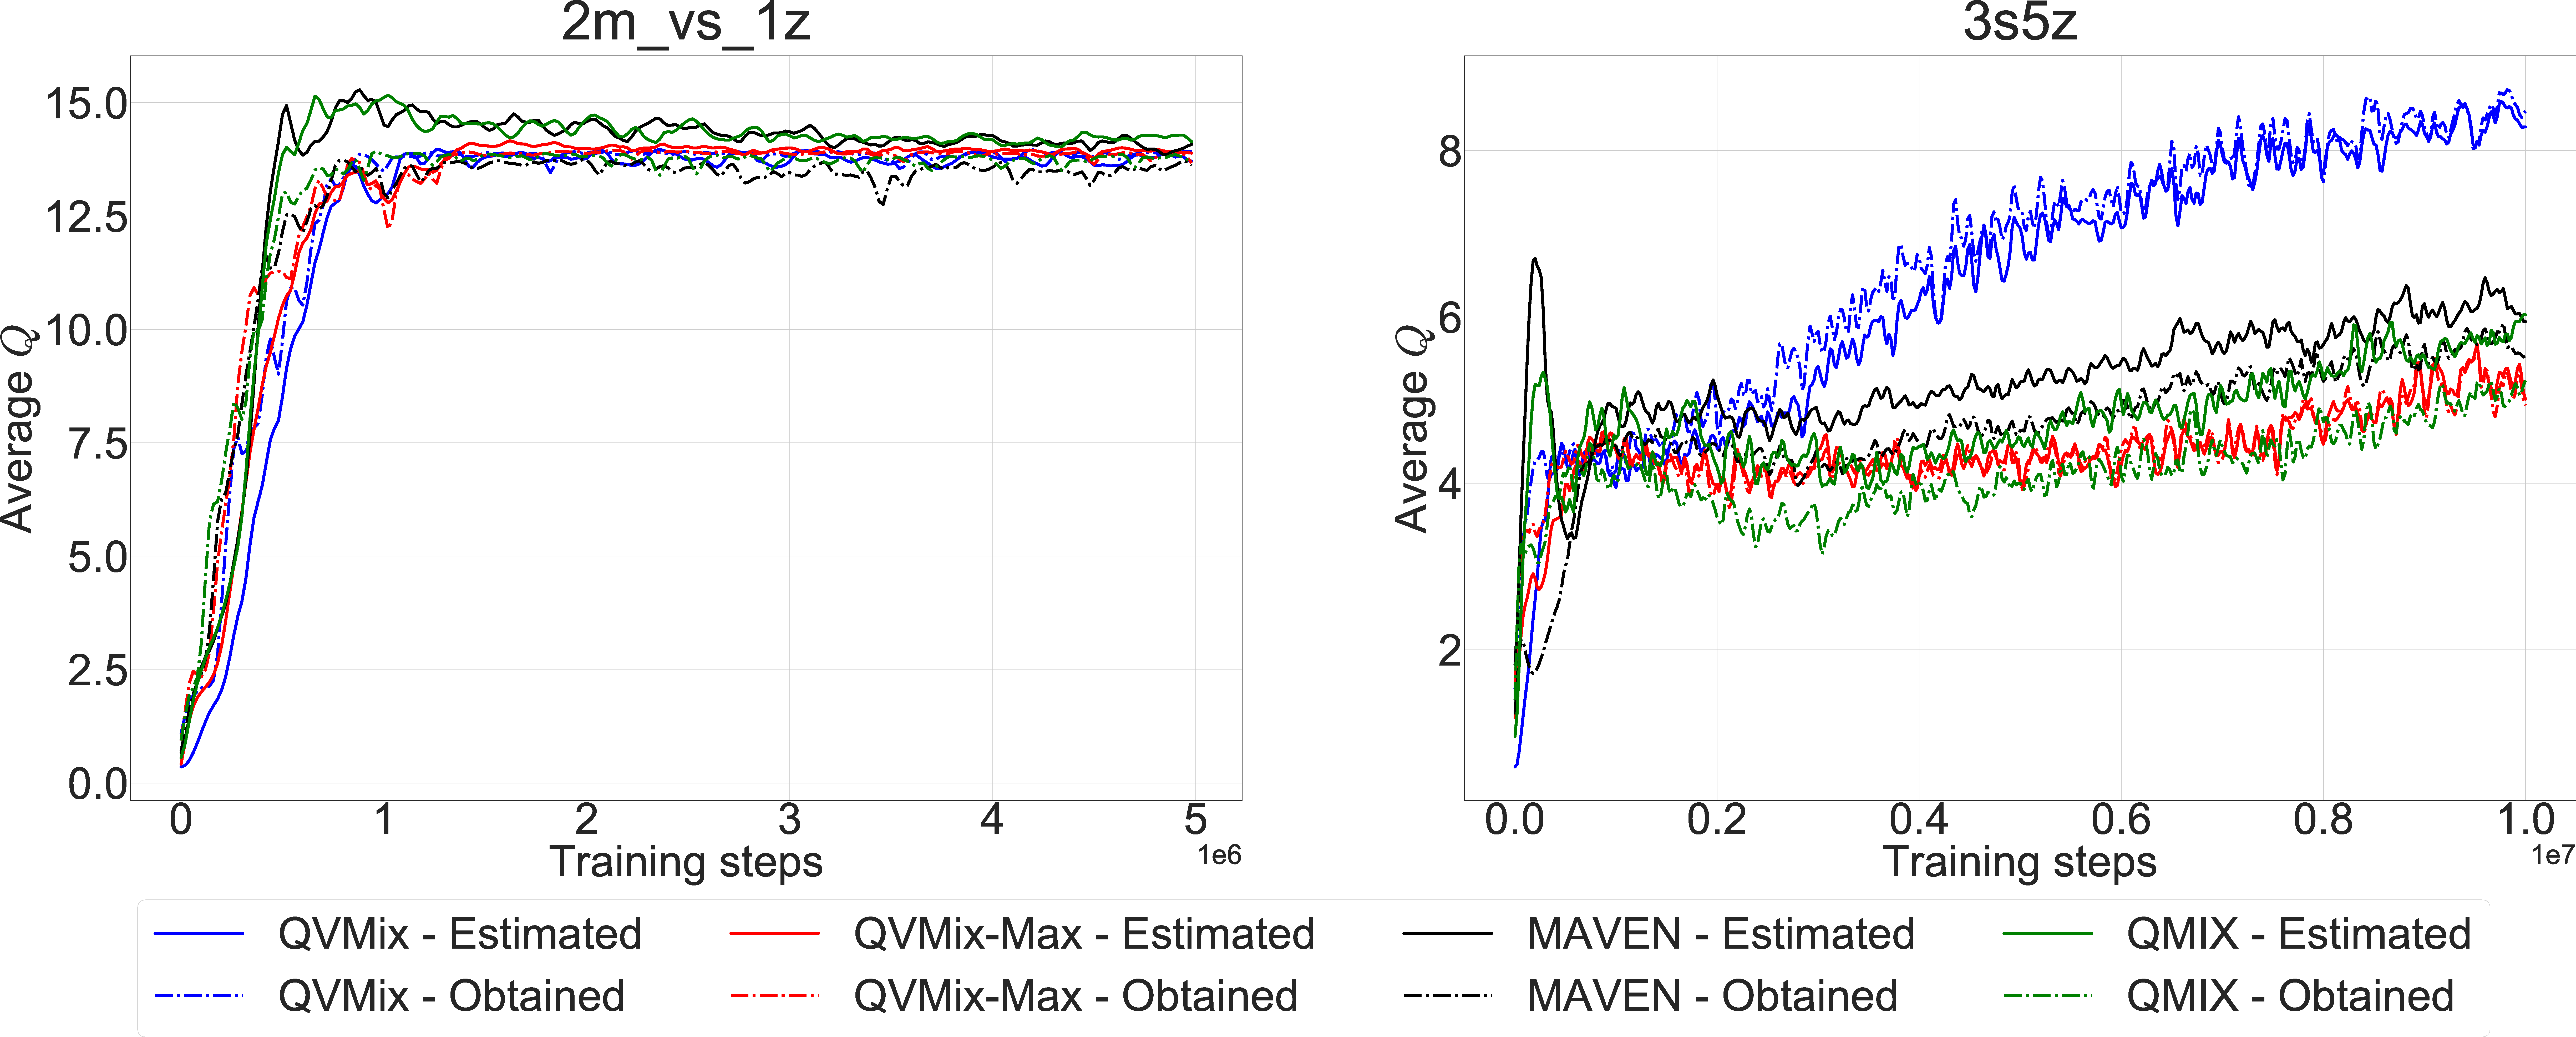
\includegraphics[width=\textwidth]{2m1z3s5zQ.pdf}
    \caption{QVMix overestimation comparison.}
\end{figure}
\blfootnote{Leroy, P., Ernst, D., Geurts, P., Louppe, G., Pisane, J.,  Sabatelli, M. (2020). QVMix and QVMix-Max: Extending the Deep Quality-Value Family of Algorithms to Cooperative Multi-Agent Reinforcement Learning}
\end{frame}


\begin{frame}{Cooperative: Policy-based methods in CTDE}
Naive learner: Independent Actor-Critic (IAC)\\
$\rightarrow$ Each agent learns its actor and critic independently.
\vfill
Two possible critics:
\begin{itemize}
\vfill
    \item IAC-V:  $A(\tau_t, u_t; \phi) = r + \gamma V(\tau_{t+1}; \phi) - V(\tau_t; \phi)$.
    \vfill
    \item IAC-Q:  $A(\tau_t, u_t; \phi) = Q(\tau_t, u_t; \phi) - \sum_{u^a}\pi_\theta(\tau_t, u^a)Q(\tau_t, u^a; \phi)$.
\end{itemize}
\vfill
Problem: How to benefit from centralised information such as $s_t$?

\vfill

\blfootnote{Foerster, J., Farquhar, G., Afouras, T., Nardelli, N.,  Whiteson, S. (2018, April). Counterfactual multi-agent policy gradients. }
\end{frame}

\begin{frame}{Cooperative: COMA}
Problem: How to benefit from centralised information such as $s_t$?
\vfill
Solutions proposed by Foerster, et. al. (2018) (COMA):
\begin{itemize}
    \item Critic is only used during training.
    \item $\rightarrow$ Centralised critic that computes the advantage based on $s_t$.
\end{itemize}

\begin{equation*}
    A(s_t,u^a_t; \phi) = r_t + \gamma V(s_{t+1}; \phi) - V(s_t; \phi)
\end{equation*}

\vfill

Problems: 
\begin{itemize}
    \item Based on global rewards $r_t$.
    \item The centralised critic does not solve the credit assignment problem.
\end{itemize}
\vfill

\end{frame}
\begin{frame}{Cooperative: COMA}

Solution: use a counterfactual baseline.
\vfill
\begin{itemize}
    \item Inspired from difference reward: 
    \vfill
    $D^a=r(s, \bm{u}) - r(s, (\bm{u}^{-a}, c^a))$
    \vfill
    The common reward $r(s, \bm{u})$ is compared to a reward obtained when agent $a$ executes a default action $c^a$, actions of other agents ($\bm{u}^{-a}$) unchanged.
    \vfill
    \item Any action $u^a$ that maximises $r(s, \bm{u})$ also maximises $D^a$.
    \vfill
    \item Problems:
    \begin{enumerate}
        \item A simulator is required to obtain $r(s, (\bm{u}^{-a}, c^a))$, but these can be approximated.
        \item One needs to decide which action is $c^a$.
    \end{enumerate}
\end{itemize}

\end{frame}

\begin{frame}{Cooperative: COMA}
 Foerster, et. al. (2018) overcomes these problems with a centralised critic that computes difference rewards by learning $Q(s, \bm{u})$.
\vfill
For each agent $a$, the advantage is:
$$ A^a(s, \bm{u}) = Q(s, \bm{u}) - \sum_{u'^{a}} \pi^a(u'^{a}|\tau^a) Q(s,(\bm{u^{-a}},u'^{a}))  $$
\vfill
Problem: $(|\mathcal{U}_1|*...*|\mathcal{U}_n|)$ $Q$ values must be computed.
\begin{itemize}
    \item In practice, a $Q$ network has one ouput for each possible action.
    \item Here, this leads to $|\mathcal{U}_1|*...*|\mathcal{U}_n|$ outputs which is impractical.
    \item COMA solution: the critic takes as input $u^{-a}$ and computes only $|\mathcal{U}_a|$ outputs.
\end{itemize}
\vfill
Note that this method is only possible for discrete action spaces, while it is possible to evaluate $\sum_{u'^{a}} \pi^a(u'^{a}|\tau^a) Q(s,(\bm{u^{-a}},u'^{a}))$ with Monte Carlo or Gaussian policies in continuous action spaces.
\end{frame}

\begin{frame}{Cooperative: COMA architecture}
\begin{figure}
    \centering
    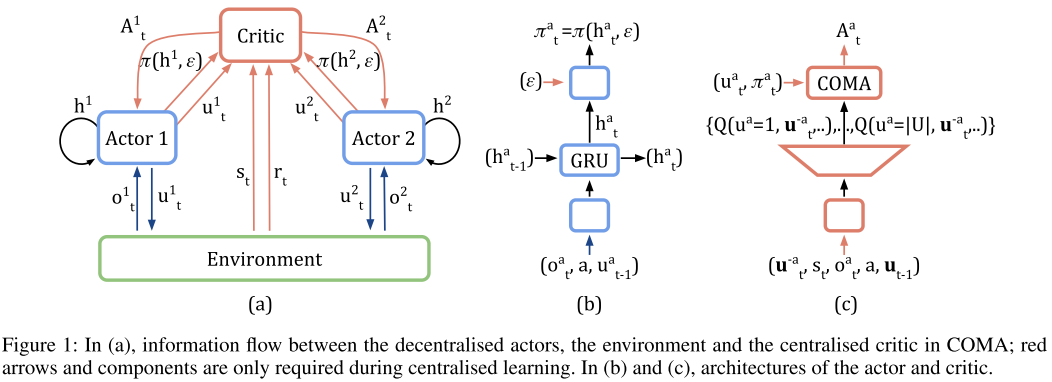
\includegraphics[scale=0.33]{coma_architecture.png}
    \caption{COMA architecture.}
\end{figure}
\blfootnote{Foerster, J., Farquhar, G., Afouras, T., Nardelli, N.,  Whiteson, S. (2018, April). Counterfactual multi-agent policy gradients. }
\end{frame}

\begin{frame}{Cooperative: COMA results}
\begin{figure}
    \centering
    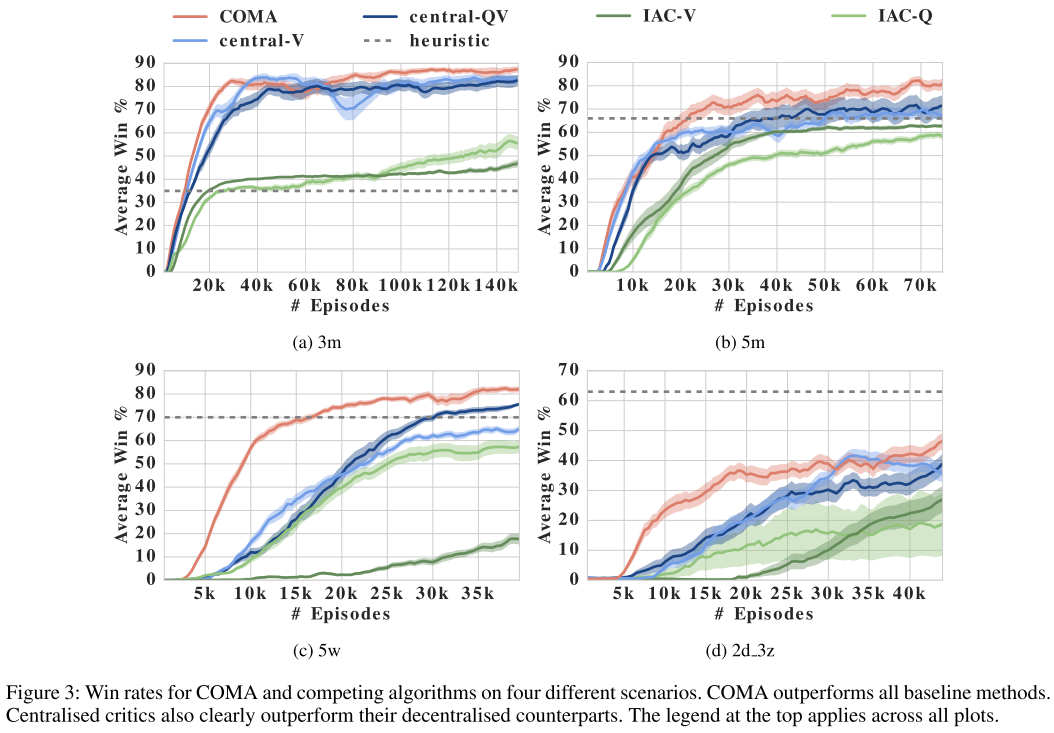
\includegraphics[scale=0.26]{coma_results.png}
\end{figure}
\blfootnote{Foerster, J., Farquhar, G., Afouras, T., Nardelli, N.,  Whiteson, S. (2018, April). Counterfactual multi-agent policy gradients. }
\end{frame}

\begin{frame}{Cooperative: COMA vs QMIX}
\begin{figure}
    \centering
    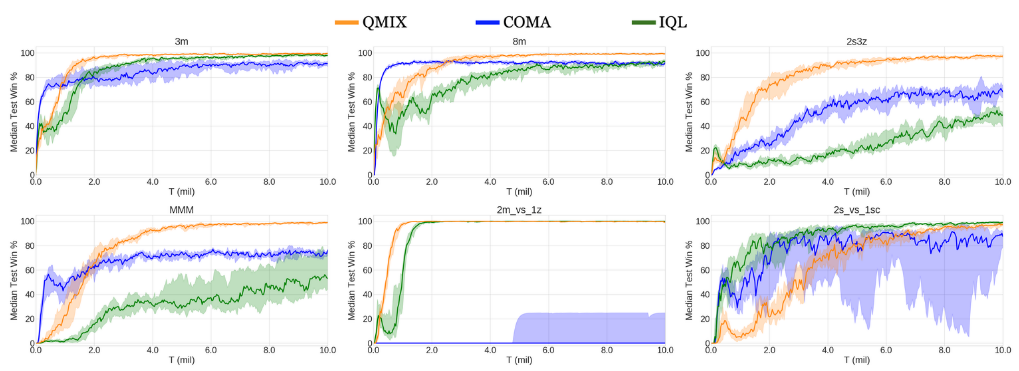
\includegraphics[scale=0.34]{coma_vs_qmix.png}
    \caption{Median win rates for QMIX, COMA, and IQL on easy SMAC scenarios.}
\end{figure}
\blfootnote{Samvelyan, M., Rashid, T., De Witt, C. S., Farquhar, G., Nardelli, N., Rudner, T. G., ...  Whiteson, S. (2019). The starcraft multi-agent challenge. }
\end{frame}

\begin{frame}{Cooperative: more methods}
\begin{itemize}
    \item MAVEN: Multi-agent variational exploration.
    \vfill
    \item QTRAN: Learning to factorize with transformation for cooperative multi-agent reinforcement learning.
    \vfill
    \item QPLEX: Duplex Dueling Multi-Agent Q-Learning.
    \vfill
    \item LIIR: Learning individual intrinsic reward in multi-agent reinforcement learning.
    \vfill
    \item MADDPG: Multi-Agent Actor-Critic for Mixed Cooperative-Competitive Environments.
    \vfill
    \item MAAC: Actor-Attention-Critic for Multi-Agent Reinforcement Learning
    \vfill
    \item FACMAC: Factored Multi-Agent Centralised Policy Gradients
    \vfill
    \item HATRPO, HAPPO: Trust Region Policy Optimisation in Multi-Agent Reinforcement Learning.
\end{itemize}
\end{frame}

\begin{frame}{Cooperation: Infrastructure Management Planning}
An application for CTDE methods:
\begin{itemize}
\item Managing infrastructure can be performed with RL and MARL.

\item Goal: Decide of inspection and repair actions over time to reduce costs and risks to maintain a system.

\item This can be applied to any type of system: civil, maritime, transportation, and urban management setting.

\item In this work: simulated deterioration and off-shore wind turbines.

\item Compared against an expert rule-based heuristic policy.

\end{itemize}

\blfootnote{
P Leroy, PG Morato, J Pisane, A Kolios, D Ernst (2023) IMP-MARL: a suite of environments for large-scale infrastructure management planning via MARL - Advances in Neural Information Processing Systems 36 (NeurIPS 2023) Datasets and Benchmarks Track 
}
\end{frame}

\begin{frame}{Cooperative: IMP}
    \begin{figure}
        \centering
        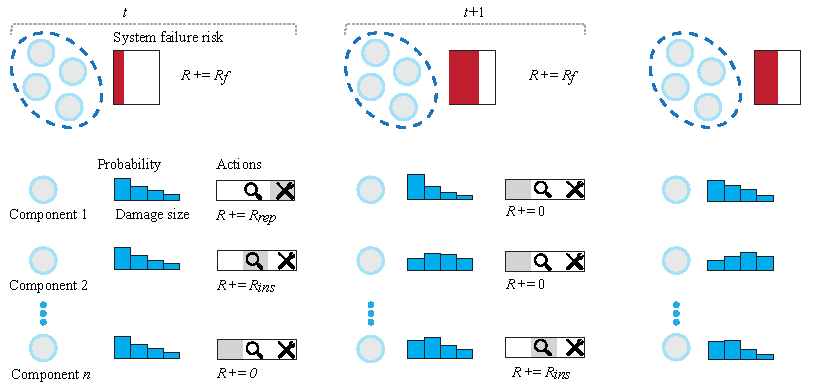
\includegraphics[width=\textwidth]{imp_intro.pdf}
        \caption{Overarching representation of an infrastructure management planning (IMP) problem.}
    \end{figure}
\end{frame}


\begin{frame}{Cooperative: IMP variations}
\begin{figure}
\begin{subfigure}[t]{0.53\textwidth}
\centering
    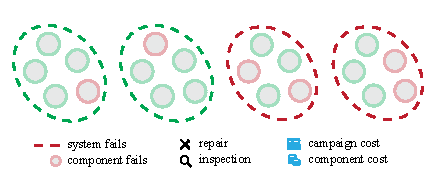
\includegraphics[width=1\linewidth]{fig2_mul/environments_v2_a.pdf}
    \caption{A k-out-of-n system environment.}
    \label{fig:env_categories_1}
\end{subfigure}%
\begin{subfigure}[t]{0.47\textwidth}
\centering
    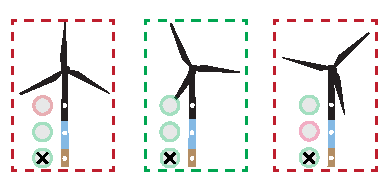
\includegraphics[width=1\linewidth]{fig2_mul/environments_v2_b.pdf}
    \caption{An offshore wind farm environment.}
    \label{fig:env_categories_2}
\end{subfigure}
%
\begin{subfigure}[t]{0.53\textwidth}
\centering
    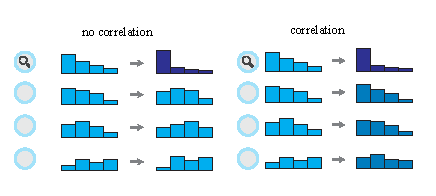
\includegraphics[width=\linewidth]{fig2_mul/environments_v2_c.pdf}
    \caption{Uncorrelated and correlated initial damage distribution.}
    \label{fig:env_categories_3}
\end{subfigure}%
\begin{subfigure}[t]{0.47\textwidth}
\centering
    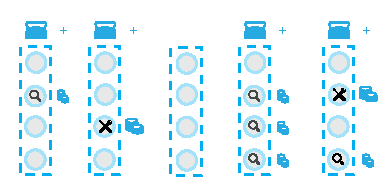
\includegraphics[width=1\linewidth]{fig2_mul/environments_v2_d.pdf}
    \caption{A campaign cost environment.}
    \label{fig:env_categories_4}
\end{subfigure}
\caption{
Visual representation of available IMP-MARL environment sets and options.}
\end{figure}
\end{frame}


\begin{frame}{Cooperative: IMP definition}
State and observations:
\begin{itemize}
    \item Belief on the deterioration state of the part.
    \item Typically the discredited probabilities on a crack size.
    \item Belief is updated with precision depending on whether or not you inspected a component of the system. 
\end{itemize}
Actions: 
\begin{enumerate}
    \item Do-nothing
    \item Inspect
    \item Replace/repair
\end{enumerate}
Reward:
\begin{equation}
     \sum_{t=0}^{T-1} \gamma^t \left[ R_{t,f}+ \sum_{a=1}^n \left({R_{t,ins}^a} + {R_{t,rep}^a}\right)+R_{t,camp} \right]
    \label{eq:totalcost}
\end{equation}
Failure cost is $R_f = c_F \times p_{Fsys}$ encompassing economic, environmental, and societal losses.
\end{frame}


\begin{frame}{Cooperative: IMP performance}
\captionsetup{font=scriptsize}
    \begin{figure}
    \centering
    \includegraphics[width=.9\textwidth]{boxplot_perc_limit_up.pdf}
\caption{Performance as normalised discounted rewards with respect to expert-based heuristic policies in all IMP environments, H referring to the heuristics result.
Every boxplot gathers the best policies from each of 10 executed training realisations, indicating the 25th-75th percentile range, median, minimum, and maximum obtained results.
%The coloured boxplots are grouped per method, vertically arranging environments with an increasing number of $n$ agents, as indicated in the top-left legend boxes.
Note that the results are clipped at -100\%.
}
\label{fig:imp_results}
\end{figure}

\end{frame}

\begin{frame}{Cooperative: IMP performance}
\captionsetup{font=scriptsize}
    \begin{figure}
    \centering
    \includegraphics[width=.9\textwidth]{boxplot_perc_limit_down.pdf}
\caption{Performance as normalised discounted rewards with respect to expert-based heuristic policies in all IMP environments, H referring to the heuristics result.
Every boxplot gathers the best policies from each of 10 executed training realisations, indicating the 25th-75th percentile range, median, minimum, and maximum obtained results.
%The coloured boxplots are grouped per method, vertically arranging environments with an increasing number of $n$ agents, as indicated in the top-left legend boxes.
Note that the results are clipped at -100\%.
}
\label{fig:imp_results2}
\end{figure}
\end{frame}




\begin{frame}{Cooperative: Recap}
\begin{itemize}
    \item Dec-POMDP
    \vfill
    \item Value-based methods
        \begin{itemize}
        \item IQL: each agent learns without considering other agents.
        \item QMIX: factorise the $Q(s,\bm{u})$ as a function of $Q^a$ and monotonicity.
        \item QVMIX: learn both $Q$ and $V$ to reduce overestimation of $Q(s,\bm{u})$.
        \end{itemize}{}
    \vfill
    \item Policy-based methods
        \begin{itemize}
        \item IAC-V, IAC-Q: each agent learns without considering other agents and with different critics.
        \item COMA: centralised critic that computes a counterfactual baseline.
        \end{itemize}{}
    \vfill
    \item Infrastructure management planning.
\end{itemize}{}
\end{frame}

\section{Communication}
\begin{frame}{Communication}
How does the stochastic game evolve with communication?

Communication can be part of the feedback loop: agents take action and send message based on local observations and messages received. 

\begin{figure}
    \centering
    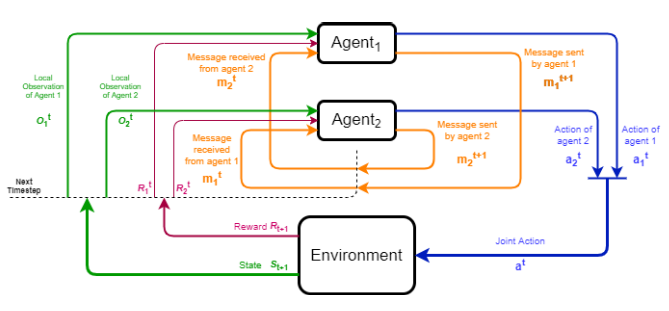
\includegraphics[scale=0.45]{com_scheme_1.png}
    \caption{Communication framework (Fombellida, A. (2020) Battlefield Coordination using Multi-Agent Reinforcement Learning)}
\end{figure}
\end{frame}

\begin{frame}{Communication: RIAL}
The two first methods are RIAL and DIAL ("Learning to communicate with deep multi-agent reinforcement learning").

\begin{itemize}
    \item Same as a Dec-POMDP, with a single reward.
    \item Agents select discrete communication action $m \in \mathcal{M}$.
    \item No communication protocol: agents must learn it (difficult).
    \item More details in the paper.
\end{itemize}
\vfill
Reinforced inter-agent learning (RIAL) is a first approach:
\begin{itemize}
    \item Each agent learns $Q^a(o^a_t, m^{-a}_{t-1}, u_t, h_{t-1})$ (called Q-Net).
    \item The network outputs is divided in $|\mathcal{U}|$ $Q^a_u$ and $|\mathcal{M}|$ $Q^a_m$ to avoid computing $|\mathcal{U}||\mathcal{M}|$ outputs.
    \item Actions and messages are chosen separately from $Q^a_u$ and $Q^a_m$ by an action selector.
\end{itemize}
\end{frame}
\begin{frame}{Communication: RIAL}
\begin{columns}
\begin{column}{0.5\textwidth}
Implementation tricks:
\begin{itemize}
    \item No more replay buffer because of non-stationarity.
    \vfill
    \item Previous action and message are inputs at next timestep.
    \vfill
    \item Parameter sharing to speed up training.
    \vfill
    \item Gradient path in red.
\end{itemize}
\end{column}
\begin{column}{0.5\textwidth}  %%<--- here  
    \begin{figure}
        \centering
        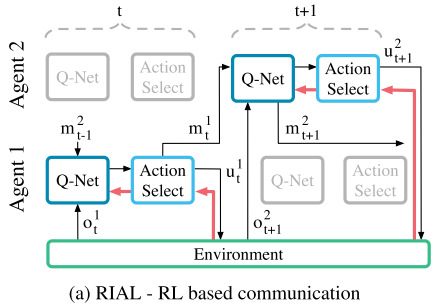
\includegraphics[scale=0.37]{rial.png}
        \caption{RIAL architecture.}
    \end{figure}
\end{column}
\end{columns}
Limitation: Agents do not provide feedbacks on messages sent by others.
    \blfootnote{Foerster, J. N., Assael, Y. M., De Freitas, N., Whiteson, S. (2016). Learning to communicate with deep multi-agent reinforcement learning.}
\end{frame}

\begin{frame}{Communication: DIAL}
Second approach: differentiable inter-agent learning (DIAL) address the feedback limitation by integrating the gradient through the communication channel.
\vfill
In RIAL, each agent is trained separately while with DIAL, CTDE is now exploited since training is performed across agents.
\vfill
Q-Net is now called C-Net and outputs:
\begin{enumerate}
    \item The $Q$ value, which is fed to the action selector.
    \item A \underline{real-valued} message.
\end{enumerate}
\vfill
Constraint: the real-valued message cannot be used during execution.
\begin{itemize}
    \item DIAL introduces a discretise/regularise unit (DRU).
    \item At training, the DRU regularises messages.
    \item At execution, the DRU discretises messages.
\end{itemize}

    
\end{frame}

\begin{frame}{Communication: DIAL}
\begin{columns}
\begin{column}{0.45\textwidth}
\begin{itemize}
    \item DIAL extends to continuous messages easily.
    \vfill
    \item DIAL perform better than RIAL.
    \vfill
    \item Results in the paper.
    \vfill
    \item This is the first attempt to learn to communicate with deep RL.
\end{itemize}

\end{column}
\begin{column}{0.6\textwidth}  %%<--- here  
\begin{figure}
    \centering
    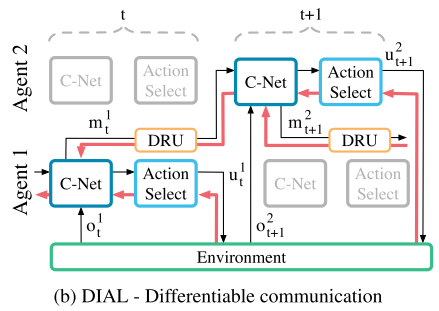
\includegraphics[scale=0.42]{dial.png}
    \caption{DIAL architecture}
\end{figure}
\end{column}
\end{columns}
\blfootnote{Foerster, J. N., Assael, Y. M., De Freitas, N., Whiteson, S. (2016). Learning to communicate with deep multi-agent reinforcement learning.}
\end{frame}

\begin{frame}{Other communication challenges}
Successor methods to DIAL and RIAL tackle other challenges with new frameworks.
\vfill
Example: agents send and receive messages before taking action, allowing multi-stage communication (several messages before action).
\vfill
Challenges and some associated papers:
\begin{itemize}
    \item Adapting to various number of agents:\\ \hspace{1.4cm} CommNet and BiCNet.
    \item Targeted communication:\\ \hspace{1.4cm} IC3Net, TarMac and ATOC.
    \item Limit the number of messages:\\ \hspace{1.4cm} SchedNet and GACML.
\end{itemize}
\end{frame}

\section{Competitive}

\begin{frame}{Competitive}
In a two player competition, the gains of one agent is equal to the loss of the other. 
\vfill
We then define a new reward function $r^{a_i}_t = R^{a_i}(s_{t+1}, s_t, u^{a_i}_t, u^{a_{-i}}_t)$.
\vfill
The goal of agent $a_i$ is to maximise this reward while for its opponent $a_{-i}$, the goal is to minimise it.
\vfill
Minimax-Q (Littman 1994) ideas:

$$V^{\pi*}(s)=\max_\pi \min_{u^{a_{-i}}} \sum_{u^{a_i} \in \mathcal{U}_i} Q^{\pi*}(s, u^{a_i}, u^{a_{-i}}) \pi(u^{a_i}|s)$$

$$Q^{\pi*}(s, u^{a_i}, u^{a_{-i}})=R^{a_i}(.) + \gamma \sum_{s'} P(s' | s,u^{a_i}, u^{a_{-i}}) V^{\pi*}(s')$$

\end{frame}

\begin{frame}{Competitive: Minimax-Q}
Littman has shown that is possible to learn these $Q$ and $V$:
\begin{figure}
    \centering
    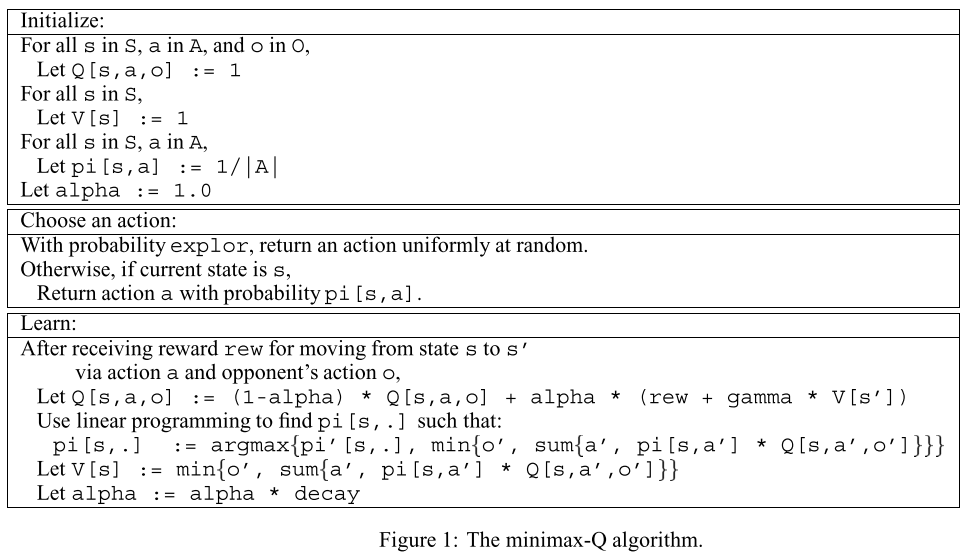
\includegraphics[scale=0.3]{minimaxQ.png}
\end{figure}

\blfootnote{Littman, M. L. (1994). Markov games as a framework for multi-agent reinforcement learning}
\end{frame}


\begin{frame}{Competitive: AlphaGo}
From AlphaGo to AlphaGo Zero: an overview of how DeepMind mastered the game of Go ($10^{360}$ possible states).
\vfill
Reminder of AlphaGo:
\begin{itemize}
    \item Two networks are trained:
    \begin{enumerate}
        \item A policy network that predicts best moves (trained in supervised learning with expert moves and improved with reinforcement learning).
        \item A value network that predicts the winner of the game.
    \end{enumerate}
    \vfill
    \item These two are combined with MCTS to provide a lookahead search and led to the first version of AlphaGo.
    \vfill
    \item "Mastering the game of Go with deep neural networks and tree search".
\end{itemize}
 \vfill
AlphaGo zero blog: \url{https://deepmind.com/blog/article/alphago-zero-starting-scratch}
\end{frame}

\begin{frame}{Competitive: MCTS reminder}

\begin{figure}
    \centering
    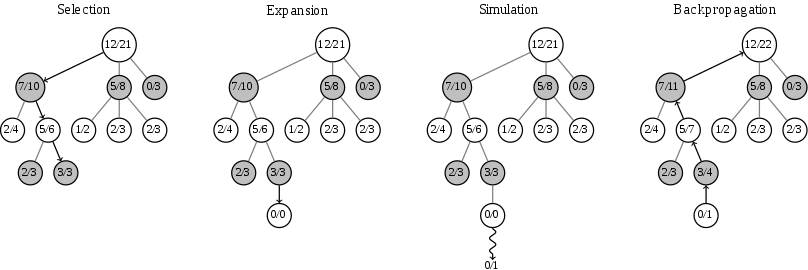
\includegraphics[width=\textwidth]{mcts.png}
    \caption{Monte Carlo tree search steps.}
    \label{fig:mcts}
\end{figure}

Reminder from Introduction to AI by Prof. Gilles Louppe: \url{https://github.com/glouppe/info8006-introduction-to-ai/}.

\end{frame}

\begin{frame}{Competitive: AlphaGo Zero}
"Mastering the game of Go without human knowledge".
\vfill
Main differences with AlphaGo:
\vfill
\begin{enumerate}
    \item No supervised learning and no human data.
    \vfill
    \item A single neural network is trained.
    \vfill
    \item Input features number is reduced (see paper for details).
    \vfill
    \item Simpler tree search that relies only on the trained network.
    \vfill
\end{enumerate}

\end{frame}

\begin{frame}{Competitive: AlphaGo Zero}
The neural network $f_\theta$:
\vfill
\begin{itemize}
    \item Input $s$: raw game board actual position and 7 previous positions.
    \vfill
    \item Outputs $(\bm{p}, v)$: a vector of probabilities and a value:
    \begin{itemize}
        \item The probability of selecting each move.
        
        \item An estimation of the probability to win from $s$.
    \end{itemize}
    \vfill
    \item Architecture details in the paper.
    \vfill
\end{itemize}
The neural network $f_\theta(s)=(\bm{p}, v)$ is trained in self-play: the agent plays lot of games against itself.
\end{frame}

\begin{frame}{Competitive: AlphaGo Zero}
To select action from a state $s$, AlphaGo Zero uses $(\bm{p}, v)$ to perform MCTS search to obtain the best moves:
 \vfill
\begin{enumerate}
    \item Perform a MCTS search to obtain probabilities $\bm{\pi}$ of selecting moves.
     \vfill
    \item They showed that $\bm{\pi}$ provides better actions than $\bm{p}$.
     \vfill
    \item Game ends with a winner $z$ that provides a sample of value $v$.
     \vfill
    \item The network is trained so that $(\bm{p}, v)$ gets closer to $(\bm{\pi}, z)$ to improve MCTS search.
\end{enumerate}
\vfill
\textbf{Note that the notation has changed: an action is represented by $a$.}
\end{frame}

\begin{frame}{Competitive: AlphaGo Zero self-play}
\begin{figure}
    \centering
    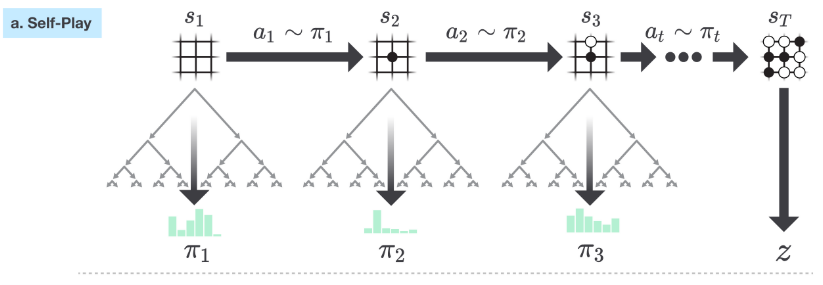
\includegraphics[scale=0.4]{alphaself.png}
    \caption{How an episode is conducted in AlphaGo Zero.}
\end{figure}
\blfootnote{Silver, D., Schrittwieser, J., Simonyan, K., Antonoglou, I., Huang, A., Guez, A., ... Hassabis, D. (2017). Mastering the game of go without human knowledge.}
\end{frame}

\begin{frame}{Competitive: AlphaGo Zero MCTS}
How $f_\theta(s)$ guides the MCTS search in AlphaGo Zero to select an action?
\begin{itemize}
    \item Each edge (s, a) stores:
    \begin{enumerate}
        \item A prior probability $P(s, a)$.
        \item A visit count $N(s, a)$.
        \item An action-value $Q(s, a)$.
    \end{enumerate}
    \item From the root, iteratively select a move that maximises:
    $$Q(s,a) + U(s, a) \: ; \: U(s, a) \propto \frac{P(s, a)}{1+N(s, a)}$$
    \item When a leaf $s'$ is reached, the network generates $f_\theta(s') = (P(s',.), V(s'))$.
    \item Each traversed edge is updated:
    \begin{enumerate}
        \item $N(s, a) = N(s, a)+1$.
        \item $Q(s, a) = 1/N(s,a) \sum_{s'|s,a\rightarrow s'} V(s')$.
    \end{enumerate}
    \item Finally, $\pi=\alpha_\theta(s) \propto N(s, a)^{1/\tau}$ ($\tau$ is a temperature parameter here).
\end{itemize}

\end{frame}

\begin{frame}{Competitive: AlphaGo Zero MCTS}
\begin{figure}
    \centering
    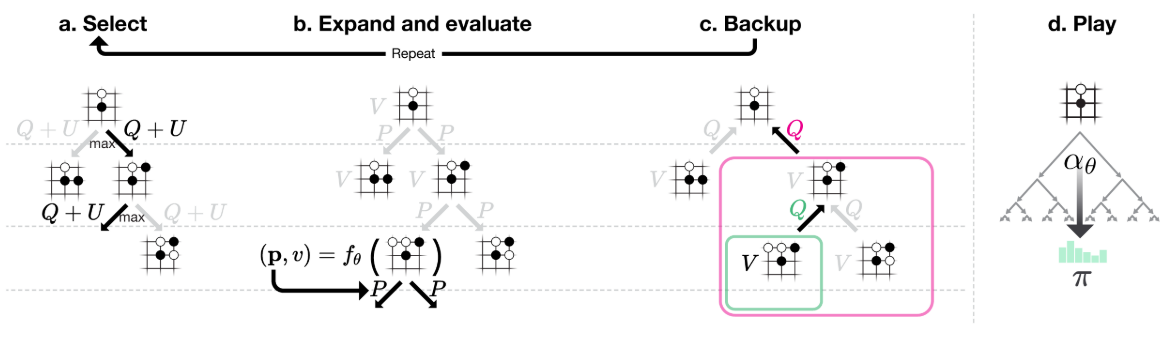
\includegraphics[scale=0.27]{alphaMCTS.png}
    \caption{MCTS in AlphaGo Zero.}
\end{figure}
\blfootnote{Silver, D., Schrittwieser, J., Simonyan, K., Antonoglou, I., Huang, A., Guez, A., ... Hassabis, D. (2017). Mastering the game of go without human knowledge.}
\end{frame}

\begin{frame}{Competitive: AlphaGo Zero training}
$$ loss = (z-v)^2 - \bm{\pi}^T log \bm{p} + c ||\theta||^2$$
\begin{figure}
    \centering
    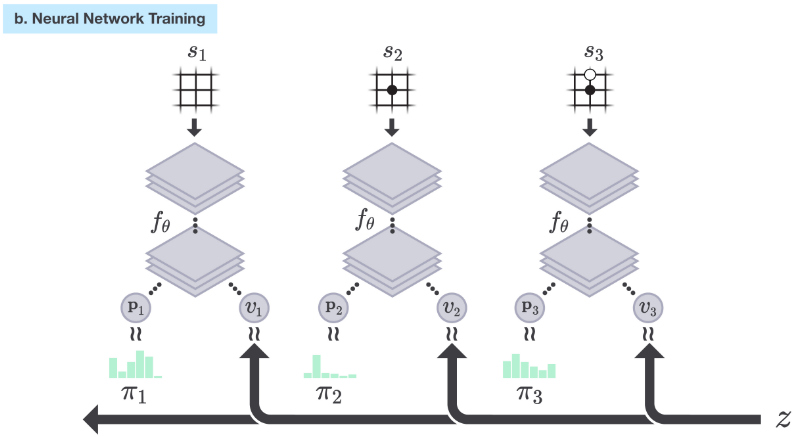
\includegraphics[scale=0.3]{alphatrain.png}
    \caption{Training in AlphaGo Zero.}
\end{figure}
\blfootnote{Silver, D., Schrittwieser, J., Simonyan, K., Antonoglou, I., Huang, A., Guez, A., ... Hassabis, D. (2017). Mastering the game of go without human knowledge.}
\end{frame}

\begin{frame}{Competitive: AlphaGo Zero numbers}
Some random numbers after $3$ days of training:
\begin{itemize}
    \item $4.9$ million games generated.
    \item $1600$ games for each MCTS ($\sim0.4s$).
    \item $700,000$ minibatches of $2,048$ states.
    \item Outperform AlphaGo Lee after $36$ hours.
    \item AlphaGo Zero on $4$ TPUs and AlphaGo Lee on $48$ TPUs.
\end{itemize}

\end{frame}


\begin{frame}{Teaser}
\centering
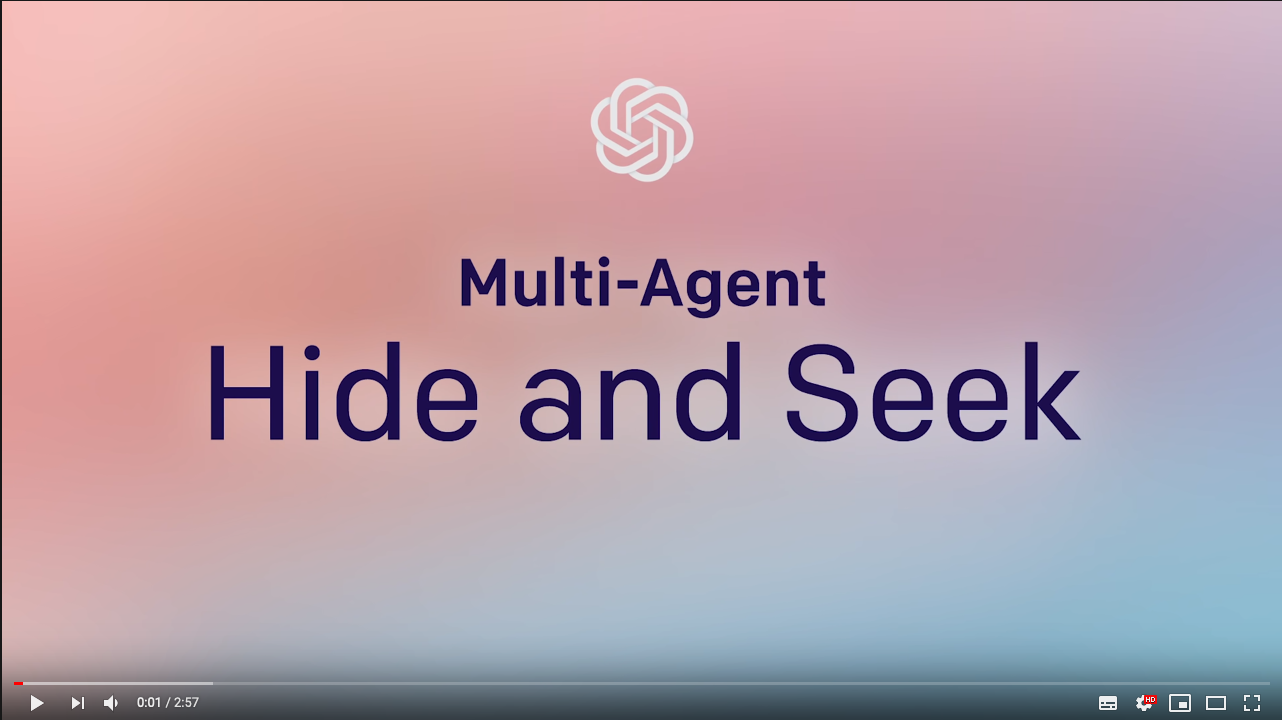
\includegraphics[scale=0.25]{teaser.png}
\url{https://www.youtube.com/watch?v=kopoLzvh5jY}
\end{frame}{}
\begin{frame}{Hide and Seek environment}

\begin{columns}
\begin{column}{0.5\textwidth}
\begin{itemize}
        \item Hiders (blue) try to avoid the line of sight of the Seekers (red).
        \item Objects can be grabbed or locked.
        \item Preparation phase: only the hiders can act initially.
    \end{itemize}{}
\end{column}
\begin{column}{0.5\textwidth}  %%<--- here
    \begin{itemize}
        \item Team-based reward.
        \item Hiders: +1 if hidden, -1 if seen.
        \item Seekers: opposite.
        \item 0 if the seekers see no one.
        \item Time limit: 240.
    \end{itemize}{}
\end{column}
\end{columns}
\begin{figure}
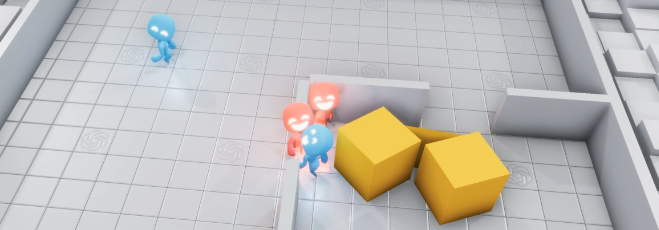
\includegraphics[scale=0.4]{hasenv.png}
\end{figure}
\end{frame}{}

\begin{frame}{Hide and Seek environment}
\begin{itemize}
    \item Action space:
    \begin{itemize}
        \item Move: discretized forces along x and y axis and torque around their z axis.
        \item Grab or lock the closest object. 2 binaries. (Only object in front of them within a small range)
        \begin{itemize}
        \item Grab: the object is bound to the agent while the boolean is True.
        \item Lock: the object is locked and cannot be moved. Unlocking is available if the agent is part of the agent team that has locked the object.
        \end{itemize}{}
        
    \end{itemize}{}
    \item Observation space:
    \begin{itemize}
        \item Position, velocity and size(or objects), in a 135 degree cone in front of the agent.
        \item "LIDAR": 30 range sensors around the agent.
    \end{itemize}{}
    \item Go to the blog!
\end{itemize}{}
    \begin{figure}
    \centering
    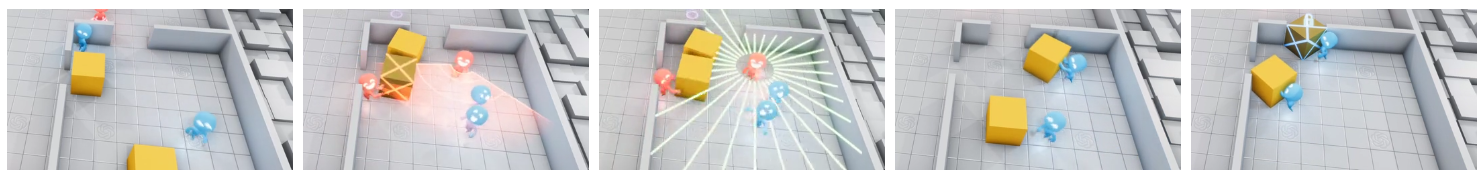
\includegraphics[scale=0.2]{hasblog1.png}
        \caption{\url{https://openai.com/blog/emergent-tool-use/}}
    \end{figure}
\end{frame}{}

\begin{frame}{Hide and Seek scenarios}
Normal environment:

\begin{columns}
\begin{column}{0.5\textwidth}
\begin{itemize}
    \item 1 to 3 hiders, 1 to 3 seekers
    \item 3 to 9 boxes (at least 3 elongated)
    \end{itemize}{}
\end{column}
\begin{column}{0.5\textwidth}  %%<--- here
    \begin{itemize}
    \item 2 movable ramps
    \item random walls and rooms
    \item random initial position
    \end{itemize}{}
\end{column}
\end{columns}
\begin{center}
    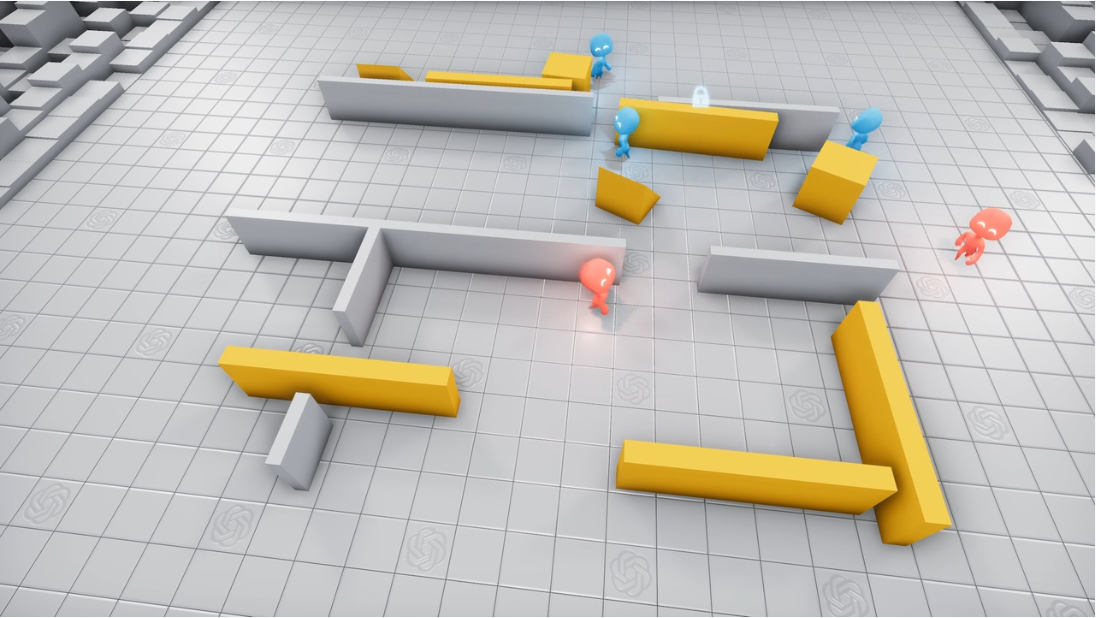
\includegraphics[scale=0.25]{normalEnv.png}
\end{center}{}
\end{frame}

\begin{frame}{Hide and Seek scenarios}
Quadrant environment:
\begin{columns}
\begin{column}{0.5\textwidth}
\begin{itemize}
    \item 2 hiders, 2 seekers
    \item 2 boxes inside the room
    \item Seekers spawn outside the room
    \end{itemize}{}
\end{column}
\begin{column}{0.5\textwidth}  %%<--- here
    \begin{itemize}
    \item 1 movable ramp that cannot be blocked
    \item 1 fixed room with 1 or 2 random doors
    \end{itemize}{}
\end{column}
\end{columns}
\begin{center}
    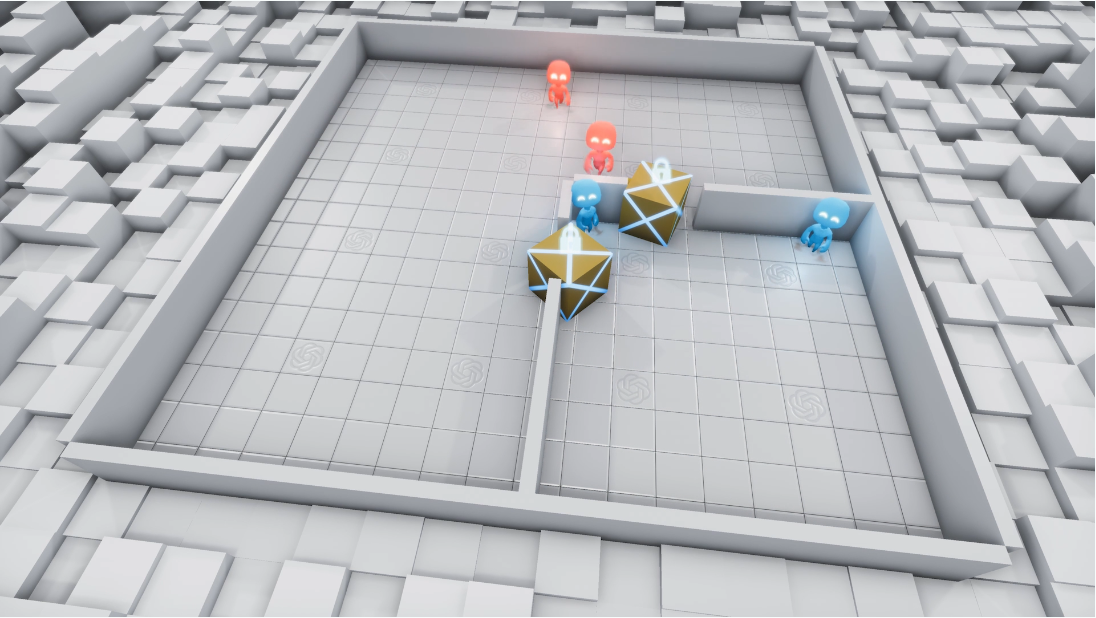
\includegraphics[scale=0.25]{quadrant.png}
\end{center}{}
\end{frame}

\begin{frame}{Hide and Seek optimization}
    \begin{itemize}
        \item Actor-Critic $\rightarrow$ 2 sets of parameters.
        \item The actor network, optimised with PPO and GAE, produces an action distribution based on the agent observations.
        \item The critic network that predicts the discounted future returns.
        \item Use centralize training, decentralized execution (CTDE).
        \begin{itemize}
            \item At training time: the critic has access to the full state to learn a centralized value function.
            \item At execution time: the policy network is used normally.
            \item No counterfactual baseline.
        \end{itemize}{}
        \item Self-play: each agent acts independently and shares the same network parameters, playing against itself.
        \item 5\% chance of using a past policy version to improve robustness.
    \end{itemize}{}
\end{frame}{}

\begin{frame}{Hide and Seek architecture}
    \begin{figure}
    \centering
    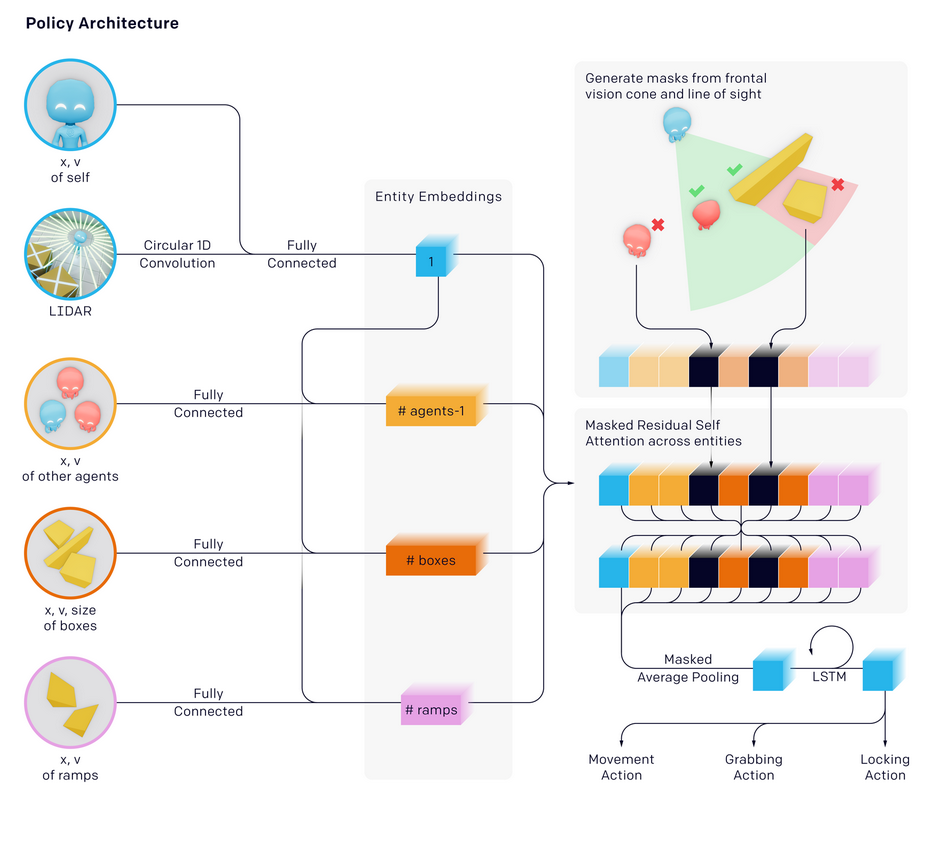
\includegraphics[scale=0.25]{hasarch.png}
    \end{figure}
\end{frame}{}

\begin{frame}{Hide and Seek entity-centric observations}
\begin{itemize}
    \item The observation is composed of different entities: agents, boxes, ramps.
    \item \textbf{The first step} is to embed each entity. Same objects are embedded with the same parameters.
    \item Self information: the concatenation of Lidar (that went through a circular 1-D convolution) with position and velocity of the agent are embedded with a fully connected layer.
    \item There are three other entities. Each one is concatenated with the embed of the self information before their own embed:
    \begin{enumerate}
        \item Other agents information ($N-1$): position and velociity.
        \item Box information (Number of boxes): position, velocity and size.
        \item Ramp information (Number of ramps): position and velocity.
    \end{enumerate}
    The number of these entities varies depending on the scenario.
\end{itemize}{}
\end{frame}{}

\begin{frame}{Hide and Seek Policy optimization}
\begin{itemize}
    \item \textbf{The second step} is to pass all embedded entities through a residual self-attention block (unobservable entities are masked away).
    \item Attention mechanisms allow to capture object-level information.
    \item "A self-attention module takes in n inputs, and returns n outputs. The self-attention mechanism allows the inputs to interact with each other (“self”) and find out who they should pay more attention to (“attention”). The outputs are aggregates of these interactions and attention scores."
    \item \textbf{The third step} is to concatenate the average-pool entities embedding with self information.
    \item \textbf{The fourth step} is to pass through a LSTM.
    \item \textbf{The last step} is to pass through the three sperate heads (one for each action type)
    \item Full parameter values are detailed in the paper.
\end{itemize}{}
\end{frame}{}

\begin{frame}{Hide and Seek Emergent behavior}
    \begin{itemize}
        \item In both scenarios, different strategies emerge as the agents train $\rightarrow$ autocurriculum. They can be seen on the blog. 
        \item In the paper, they insist on the fact that there is no incentives for agents to interact with objects, this is only a result of autocurriculum induced by the competition.
    \end{itemize}{}
        \begin{figure}
        \centering
    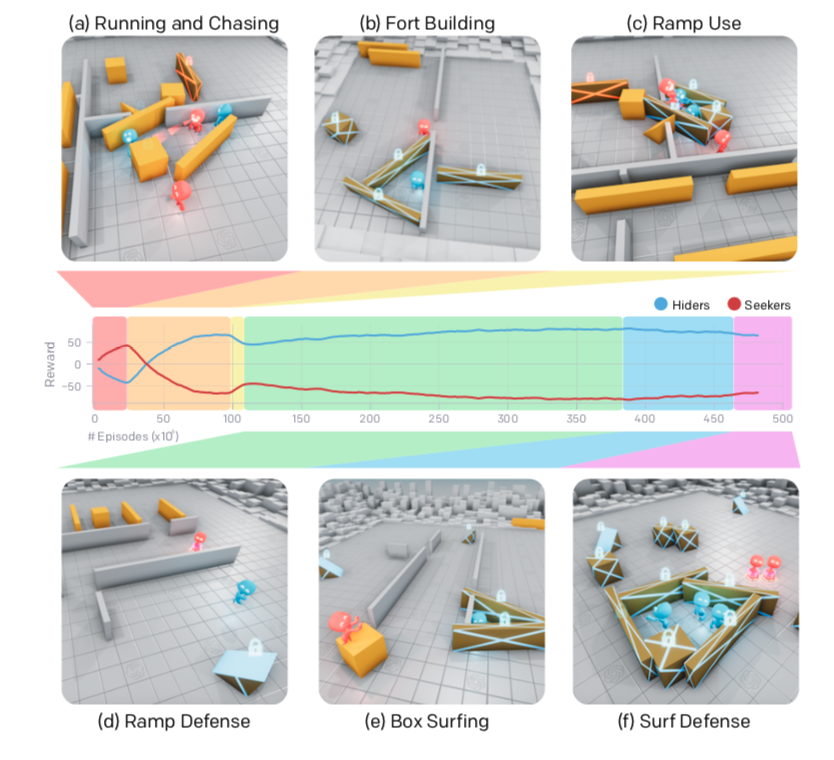
\includegraphics[scale=0.2]{Figure1.png}
    \end{figure}{}
\end{frame}{}

\begin{frame}{Hide and Seek Emergent behavior}
Tool interaction
    \begin{itemize}
        \item Agents learn to divide the labor: Against box surfing, 2 and 3 hiders lock 25\% and 36\% more boxes than a single hider.
        \item It is possible to track the stages of emergent policy with the interaction of tools in the environment.
    \end{itemize}{}
    \begin{figure}
        \centering
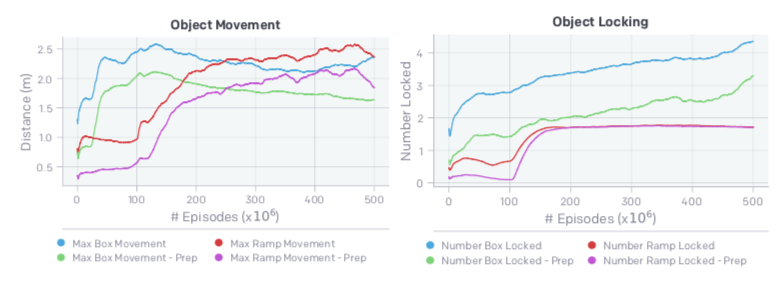
\includegraphics[scale=0.4]{Figure3.png}
    \end{figure}{}
     
\end{frame}{}

\begin{frame}{Hide and Seek Emergent behavior}
    \begin{itemize}
        \item Scale matters!
        \item In the Figure, the number of episode (blue) and time (orange) \textbf{to reach stage 4 }(ramp defense) in term of batch size.
        \item The size of batch size is the number of transition chunks.
        \item The model uses 1.6 million parameters.
    \end{itemize}{}
     
         \begin{figure}
        \centering
        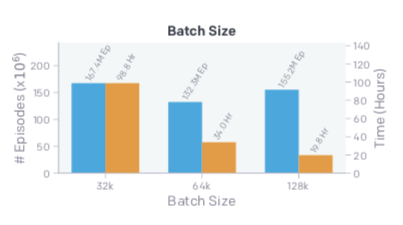
\includegraphics[scale=0.6]{Figure4.png}
    \end{figure}{}
\end{frame}{}

\begin{frame}{Hide and Seek Evaluation}
Evaluation
\vfill
    \begin{itemize}
        \item Reward in Multi-Agent is not sufficient to evaluate agents.
        
        Are agents improving evenly or have they stagnated?
        \vfill
        \item ELO score (or Trueskill) allows to establish a ranking and measures improvement compared to other policies. However, it does not differentiate adaptation and improvement of already learned skills.
        \vfill
        \item Their propose two evaluations scheme.
        \vfill
        \begin{enumerate}
            \item Comparison to intrinsic motivation.
            \vfill
            \item Inteligence tests: transfer and fine-tuning.
            \vfill
        \end{enumerate}{}
    \end{itemize}{}
\end{frame}{}

\begin{frame}{Hide and Seek Intrinsic motivation}
    \begin{itemize}
        \item \textbf{Goal?} Compare behavior learned in Hide and Seek with common unsupervised exploration techniques.
        \vfill
        \item Underlying idea: Can agent behave like human with these unsupervised exploration methods.
        \vfill
        \item Count based exploration: the agent receives reward when visiting states that has not been visited much.
        \vfill
        \item Very dependent of state representation.
        \vfill
        \item \textbf{Result}: The learned behavior is very not human-like.
        \vfill
        \item See blog results.
    \end{itemize}{}
\end{frame}{}

\begin{frame}{Hide and Seek Intelligence tests}
    \begin{itemize}
        \item \textbf{Goal?} Use transfer learning to evaluate network parameters on five new tasks.
        \item Three configuration:
        \begin{enumerate}
            \item Trained from scratch
            \item Pre-trained with Hide and Seek and fine tuned.
            \item Pre-trained with count based and fine tuned.
        \end{enumerate}{}
        \item These tests include supervised learning and reinforcement learning but are single-agent: 
        \begin{enumerate}
            \item Object counting
            \item Lock and return
            \item Sequential lock
            \item Construction from blueprint
            \item Shelter construction
        \end{enumerate}{}
        \item Notes:
        \begin{itemize}
        \item Same spaces and observation (fake hiders)
        \item Object counting task: the action heads are replaced by a classification head (7-classes representing whether 0 through 6 boxes have gone to the left)
        \end{itemize}{}
    \end{itemize}{}
\end{frame}{}

\begin{frame}{Hide and Seek Intelligence tests}
Results:
    \begin{itemize}
    \item Pre-trained with Hide and Seek configuration is better on Lock and return, Sequential lock and Construction from blueprint.
    \item Pre-trained with count-based configuration is better on Object counting.
    \item Pre-trained with Hide and Seek configuration achieves the same results as the trained from scratch configuration on Shelter construction but sligthly slower.
    \end{itemize}{}
\end{frame}{}

\begin{frame}{More intelligence tests}
Intelligence tests are performed at different phases of emergence.
\begin{figure}
    \centering
    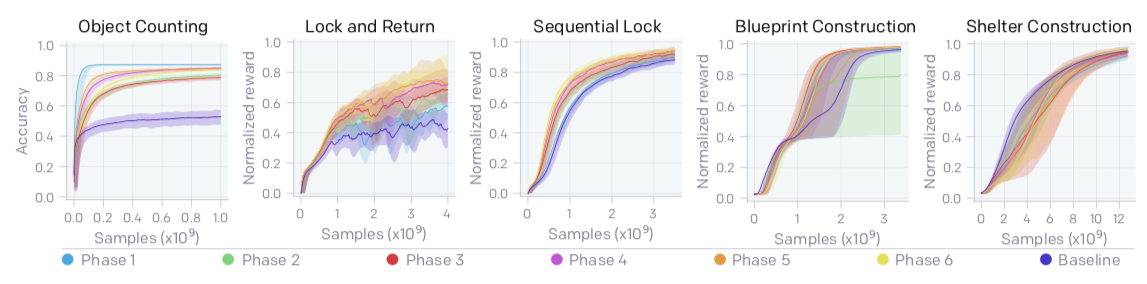
\includegraphics[scale=0.3]{FigureA5.png}
\end{figure}{}
\begin{itemize}
    \item Improves on navigation and memory as it progresses.
    \item Object counting is transient.
    \item Performance on manipulation tasks (constructions) is uncorrelated to the phases. The most surprising: policy from phase 1 performs comparably well to others.
\end{itemize}{}
\end{frame}{}

\begin{frame}{Alternative games}
Hide and Seek with food reward.
    \begin{itemize}
        \item Can eat food if:
        \begin{itemize}
            \item after preparation phase.
            \item hiders not seen by seekers.
            \item hider close and visible to the food.
        \end{itemize}{}
    \end{itemize}{}
    \begin{figure}
        \centering
        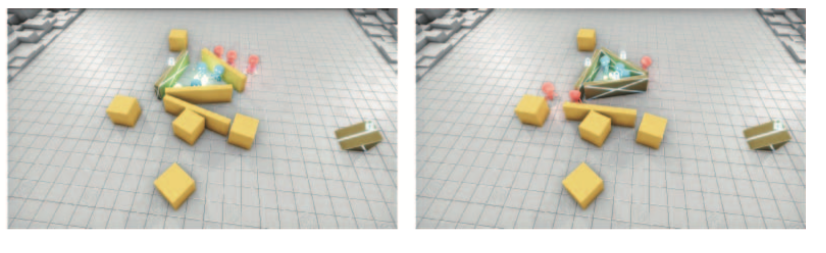
\includegraphics[scale=0.4]{FigureA6.png}
        \caption{Hide and Seek with food reward.}
    \end{figure}{}
\end{frame}{}
\begin{frame}{Alternative games}
Hide and Seek with food reward: Results.
    \begin{itemize}
        \item Incentivized to build forts around food.
        \item Four levels of skill progression (see Figure)
    \end{itemize}{}
    \begin{figure}
        \centering
        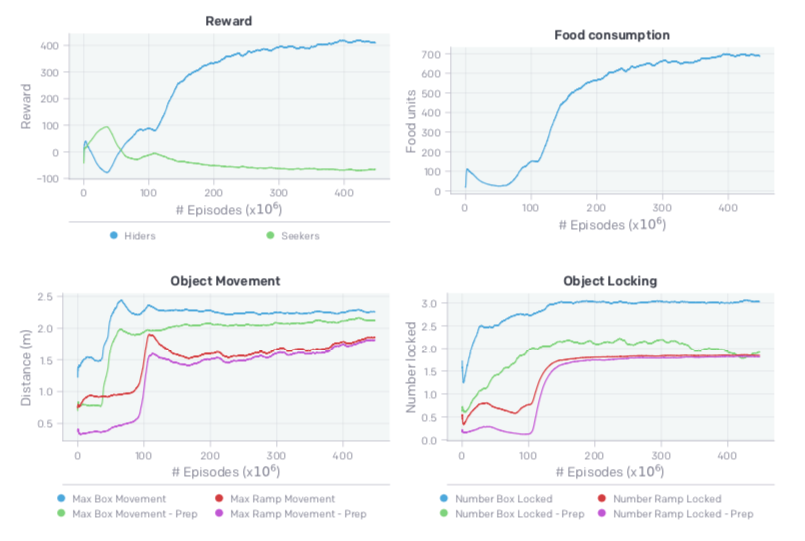
\includegraphics[scale=0.25]{FigureA7.png}
        \caption{Hide and Seek with food reward results}
    \end{figure}{}
\end{frame}{}
\iffalse
\begin{frame}{Alternative games}
Hide and Seek with dynamic food.
    \begin{itemize}
        \item Only one food that disappear when eaten.
        \item It reappears in the center of the map (in a square of length 1/5 of game area size).
        \item The hidders need to learn to build large forts.
        \item Emerge after 45 billions samples.
        \item If food region ratio is 1/6, emerge after 15 billions samples.
        \item If food region ratio is 1/4, the hiders ignore food and protect themselves.
    \end{itemize}{}
\end{frame}{}

\begin{frame}{Conclusions}
Claims:
    \begin{enumerate}
        \item Simple game rules and multi-agent competition can induce agents to learn complex strategies and skills.
        \vfill
        \item Intelligent tests, using transfer learning, can be used to evaluate learning progress and to compare agents in a same domain.
        \vfill
        \item Multi-agent autocurricula can lead to physically grounded and human-relevant behavior (in opposition to unsupervised exploration techniques).
    \end{enumerate}{}

Bonus: \href{https://openai.com/research/emergent-tool-use}{Surprising behaviors!!}
\end{frame}{}

\fi

\begin{frame}{Competitive: Other works}
Recent work has been done in competitive games:
 \vfill
\begin{itemize}
    \item Dota 2, OpenAI Five (2019): Dota 2 with large scale deep reinforcement learning.
     \vfill
    \item StarCraft 2, AlphaStar (2019): Grandmaster level in StarCraft II using multi-agent reinforcement learning.
     \vfill
    \item Quake 3 capture the flag (2019): Human-level performance in 3D multiplayer games with population-based reinforcement learning.
     \vfill
     \item Stratego ($10^{535}$ possible states): Deep Nash (2022) Mastering the game of Stratego with model-free multiagent reinforcement learning.

     
\end{itemize}
\end{frame}

\begin{frame}{Competitive: AlphaStar}
\href{https://www.deepmind.com/blog/alphastar-mastering-the-real-time-strategy-game-starcraft-ii}{Discussion on AlphaStar}
\end{frame}

\begin{frame}{Competitive: Two team markov game}
What if we have 2 symmetric teams?
    \begin{itemize}
        \item A set of $n$ agents, each one is represented by $a$ or $a_{i, j}, i \in  \{1,...,n\}, j \in \{1, 2\}$.
        \vfill
        \item A set of states $s \in \mathcal{S}$.
        \vfill
        \item An observation function $O:\mathcal{S} \times \{1,...,n\} \rightarrow \mathcal{Z}$.
        \vfill
        \item A set of action spaces $\mathcal{U}=\mathcal{U}_1 \times ... \times \mathcal{U}_n$, one per agent $u^{a_{i,j}}_{t} \in \mathcal{U}_i \forall j$.
        \vfill
        \item A transition function: $s_{t+1} \sim P(s_{t+1} | s_t, \boldsymbol{u_t})$,  $\boldsymbol{u_t}=\bigcup_{i \in \{1,..,n\},j. \in \{1,2\}} u^{a_{i,j}}_t$.
        \vfill
        \item A reward function per team:  $r^j_t = R^j(s_{t+1}, s_t, \boldsymbol{u_t})$.
        \vfill
        \item Agents store their history $\tau^a_t \in (\mathcal{Z} \times \mathcal{U})^t$.
        \vfill
        \item The goal of each agent $a_i$ is to maximize its total expected sum of (discounted) rewards $\sum_{t=0}^{T} \gamma^t r^{a_i}_t$.
    \end{itemize}{}

\end{frame}

\begin{frame}{Two team markov game}
How to train a team of agents to compete?\\
Train against multiple evolving strategies!

\begin{itemize}
    \item Teams are trained with CTDE methods: QMIX, QVMix and MAVEN.
    \item Teams are trained with three different learning scenarios: \begin{enumerate}
        \item Against a stationary strategy,
        \item Self-play,
        \item Within a population of training teams.
    \end{enumerate}
    \item New Competitive StarCraft Multi-Agent Challenge.
    \item Teams trained with $10^7$ timesteps in 2 different environments ($3m$ and $3s5z$).
    \item Each method/scenario pair has been executed 10 times.
    \item Evaluation is performed with Elo scores and win rates.

\end{itemize}
\blfootnote{Leroy, P., Pisane, J., Ernst, D. (2022). Value-based CTDE Methods in Symmetric Two-team Markov Game: from Cooperation to Team Competition.}
\end{frame}

\begin{frame}{Two team markov game: Elo score }
\begin{itemize}
    \item The purpose of the Elo rating system is to assign each player of a population with a rating $R$ to rank them.
    \item It is possible to compute the probability that a player will win when facing another one.
Let $R_A$ and $R_B$ be the ELO scores of player A and B, respectively, then $E_A$ = proba A wins. 

\begin{equation}
    E_A=\frac{10^{R_A/400}}{10^{R_A/400} + 10^{R_B/400}}
    \text{ and }
    E_B=\frac{10^{R_B/400}}{10^{R_A/400} + 10^{R_B/400}}
\end{equation}
One can see that $E_A + E_B = 1$.
\item $400$ is a parameter: if the Elo score of player A is 400 points above that of B, it has a ten-times greater chance of defeating B.

\item $S_A$ is equal to $1$ for a win, $0$ for a loss and $0.5$ for a draw.

\item New score is 
\begin{equation}
    \label{eq:elo_update}
    R'_A = R_A + cst * (S_A - E_A)
\end{equation}
where $cst$ is a constant that defines the maximum possible update of the Elo score (10 in our paper, typically 32).
\end{itemize}
\end{frame}

\begin{frame}{Two team markov game: results}
\textbf{H} = trained against heuristic,
\textbf{S} = self-play,\\
\textbf{P} = within a population,
\textbf{BP} = the 10 bests of each population.

Elo after training (Elo score obtained in different test populations):
    \begin{figure}
        \centering
        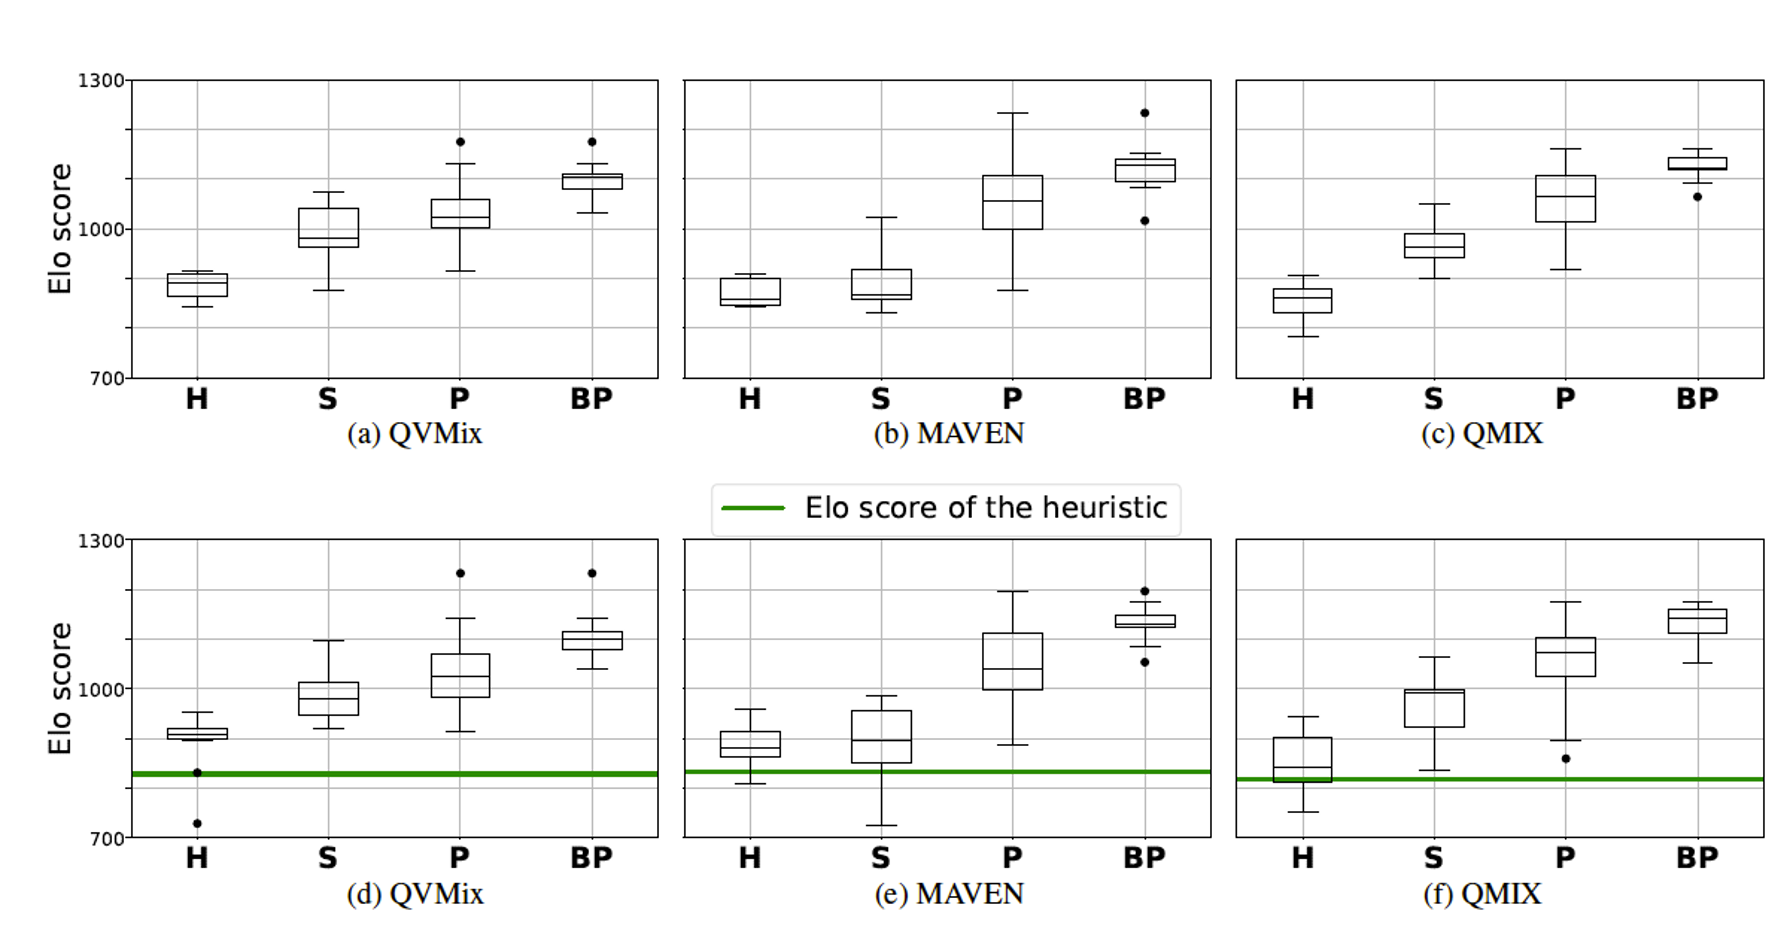
\includegraphics[width=\textwidth]{2team1.png}
    \end{figure}
\end{frame}

\begin{frame}{Two team markov game: results}
Win-rates during training against the heuristic than against themselves.
    \begin{figure}
        \centering
        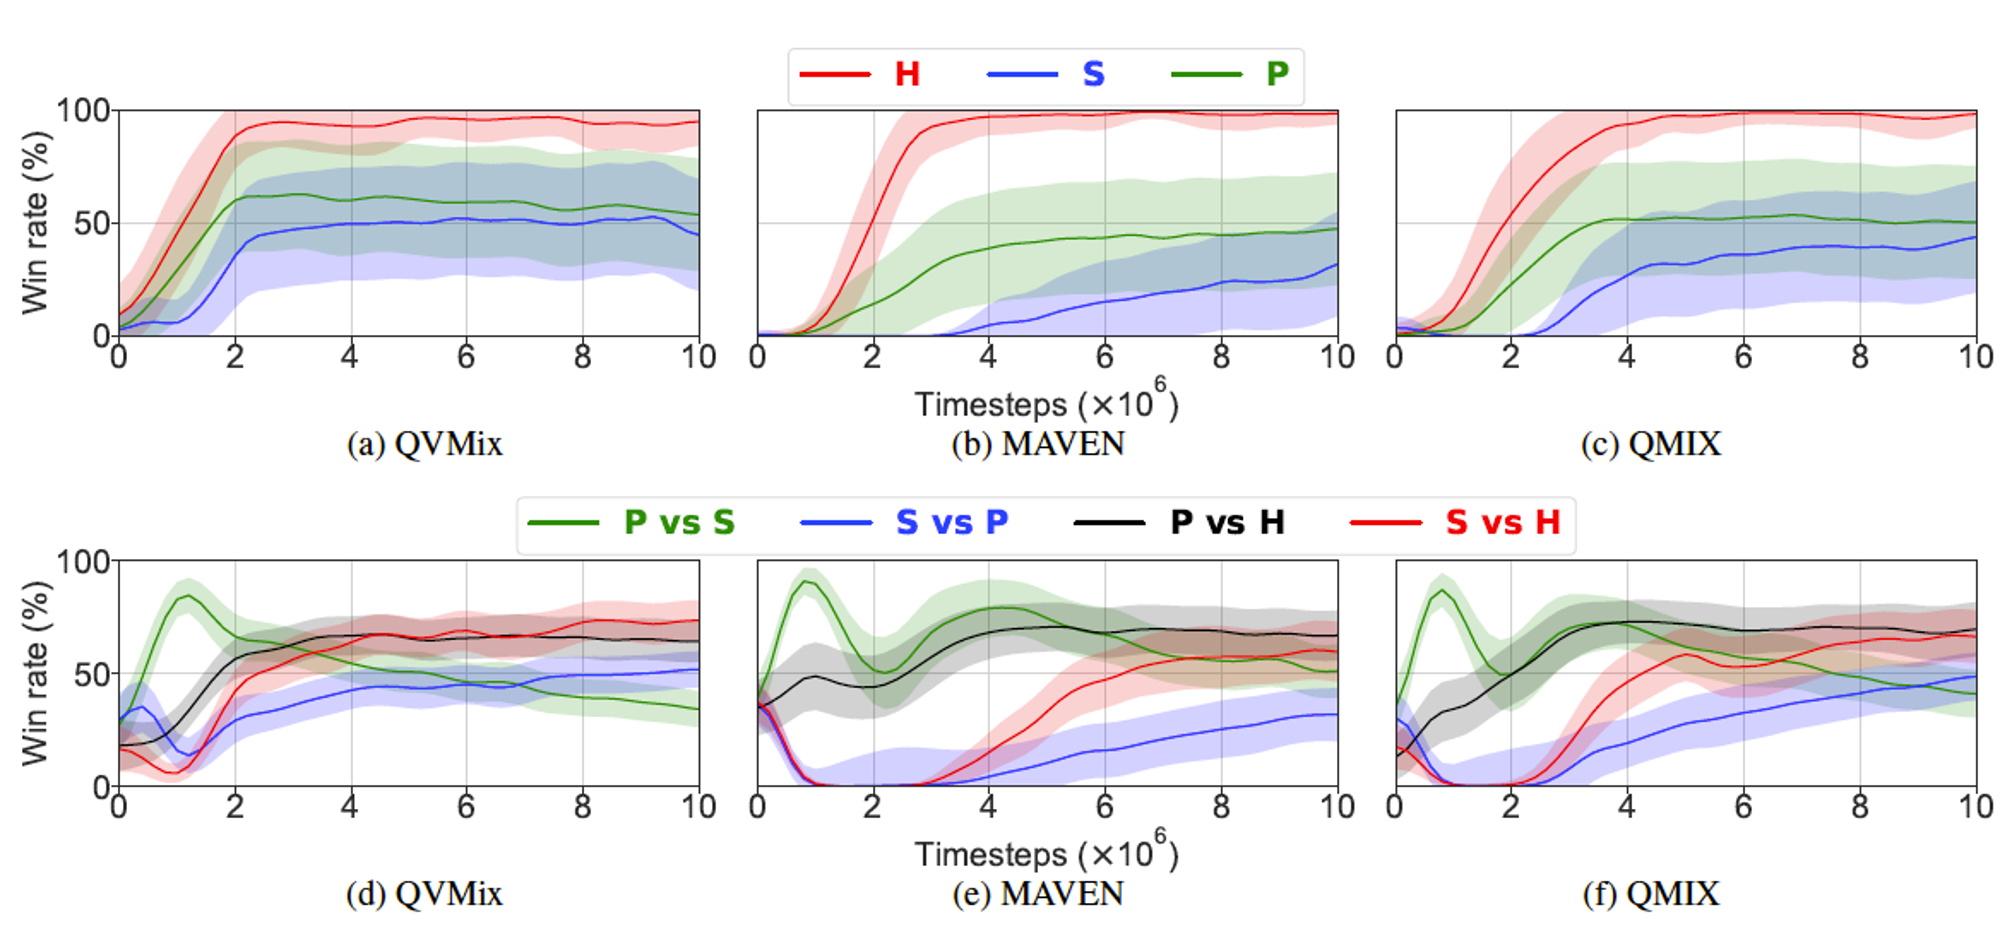
\includegraphics[width=\textwidth]{2teams2.png}
    \end{figure}
\end{frame}
\begin{frame}{Two team markov game: results}
    \begin{figure}
        \centering
        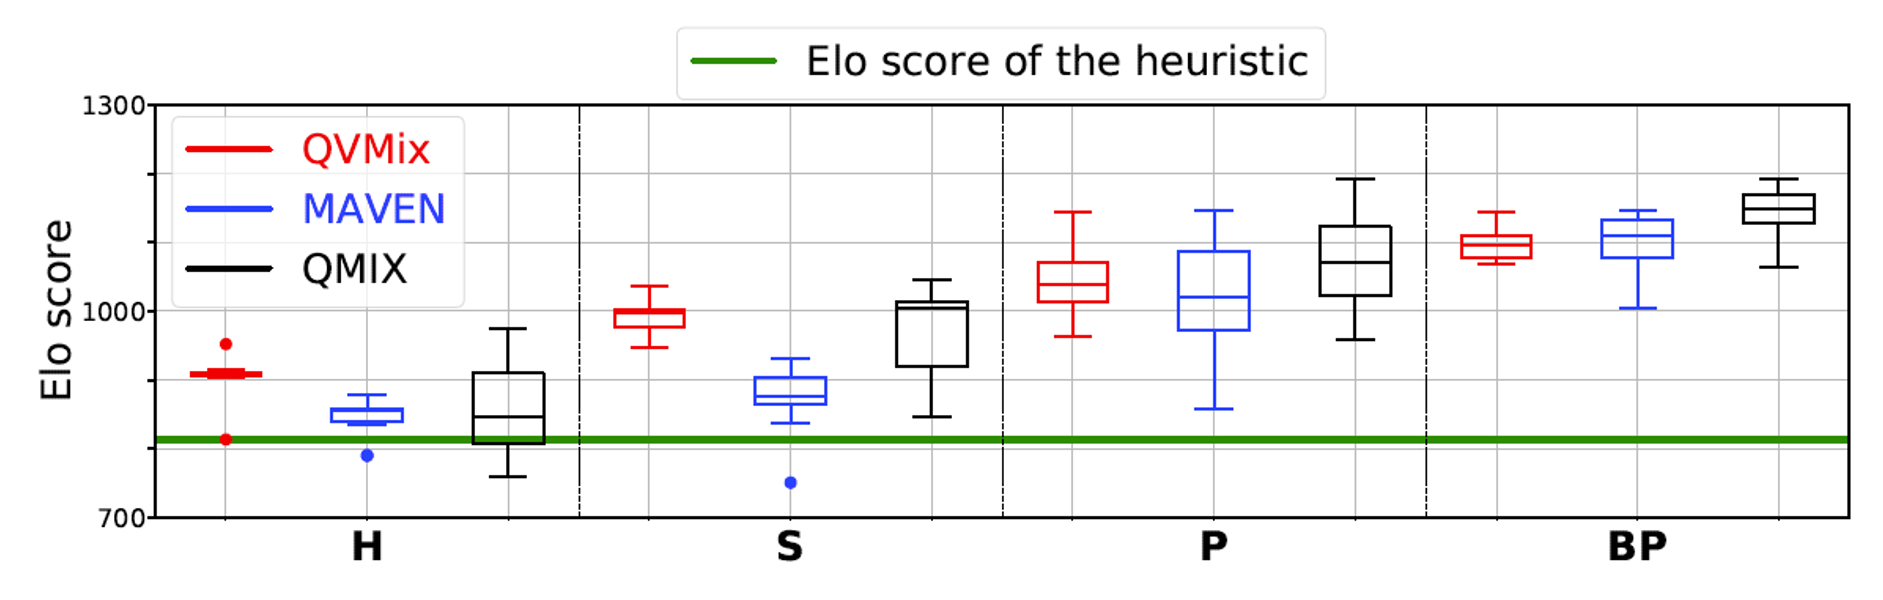
\includegraphics[width=\textwidth]{2teams3.png}
    \end{figure}
\end{frame}
\begin{frame}{Two team markov game: training duration}

\begin{figure}
    \centering
    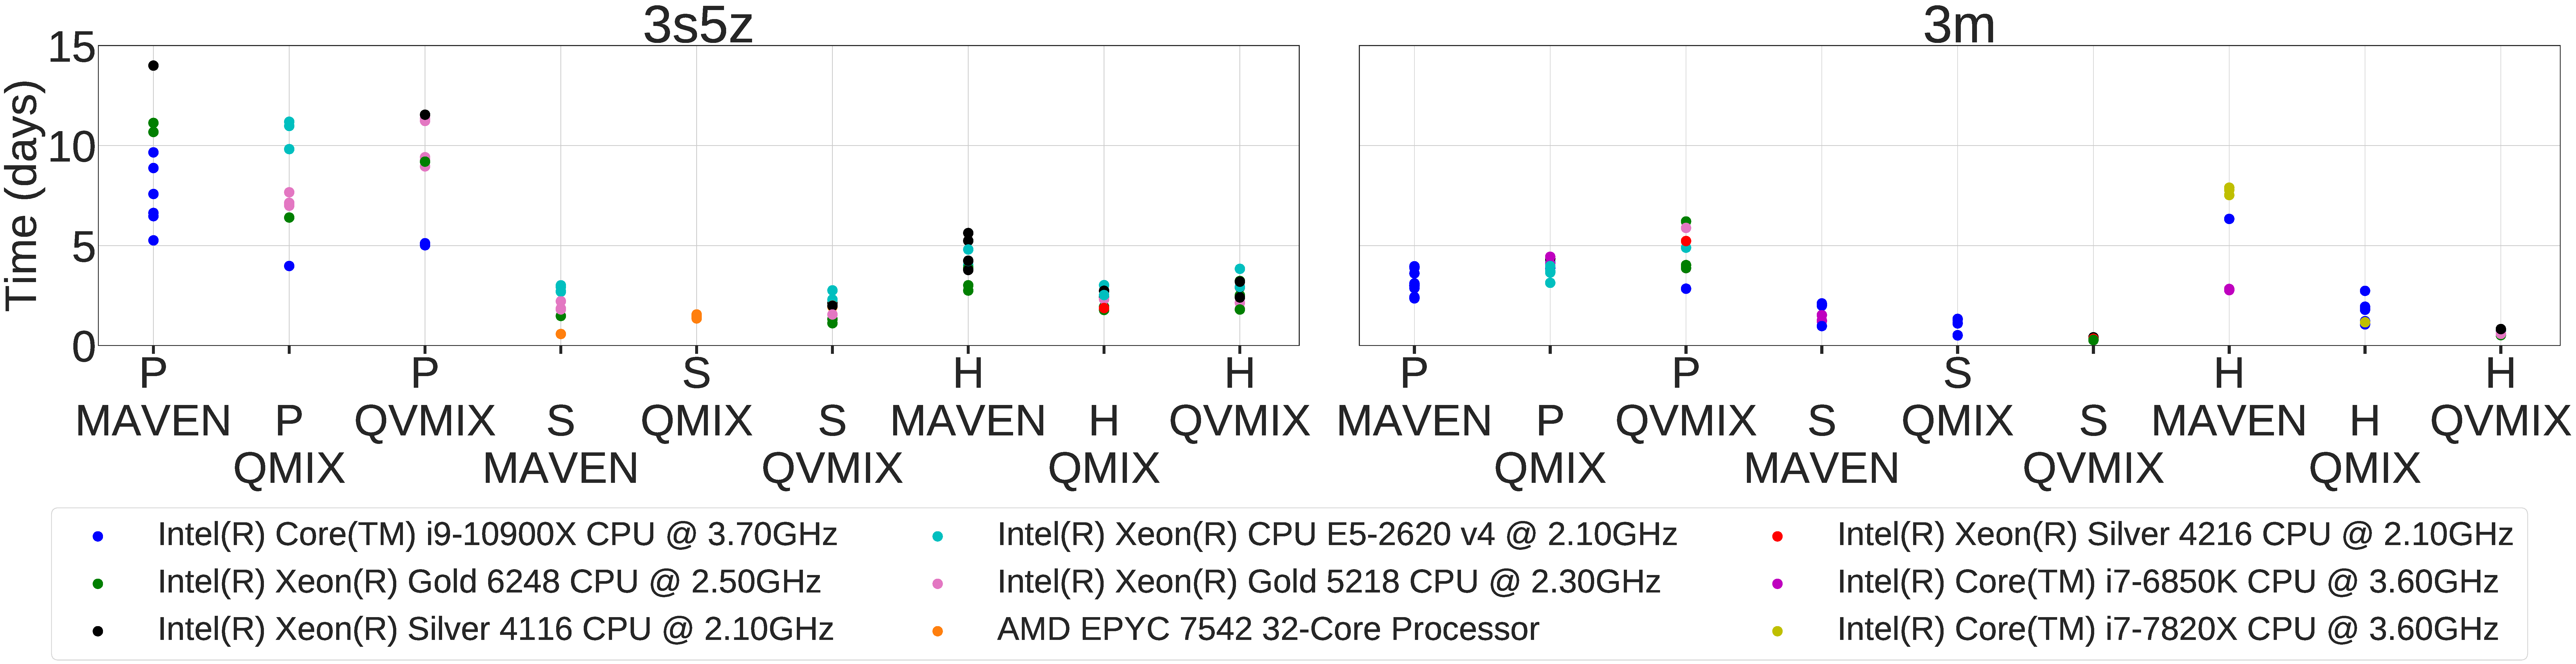
\includegraphics[width=\textwidth]{training_time.pdf}
\end{figure}
\end{frame}

\begin{frame}{Two team markov game: Conclusions}

Conclusions:
\begin{itemize}
    \item Training teams within a population of learning teams is the best learning scenario, when each team plays the same number of timesteps for training purposes.
    \vfill
    \item This is irrespective of whether or not the stationary strategy was better than all trained teams.
    \vfill
    \item  A selection procedure is required in the same training population.
\end{itemize}


\end{frame}





\section{Adversarial attacks}

\begin{frame}{Adversarial attacks}
It is possible to trick a neural network with small perturbations.
\begin{figure}
    \centering
    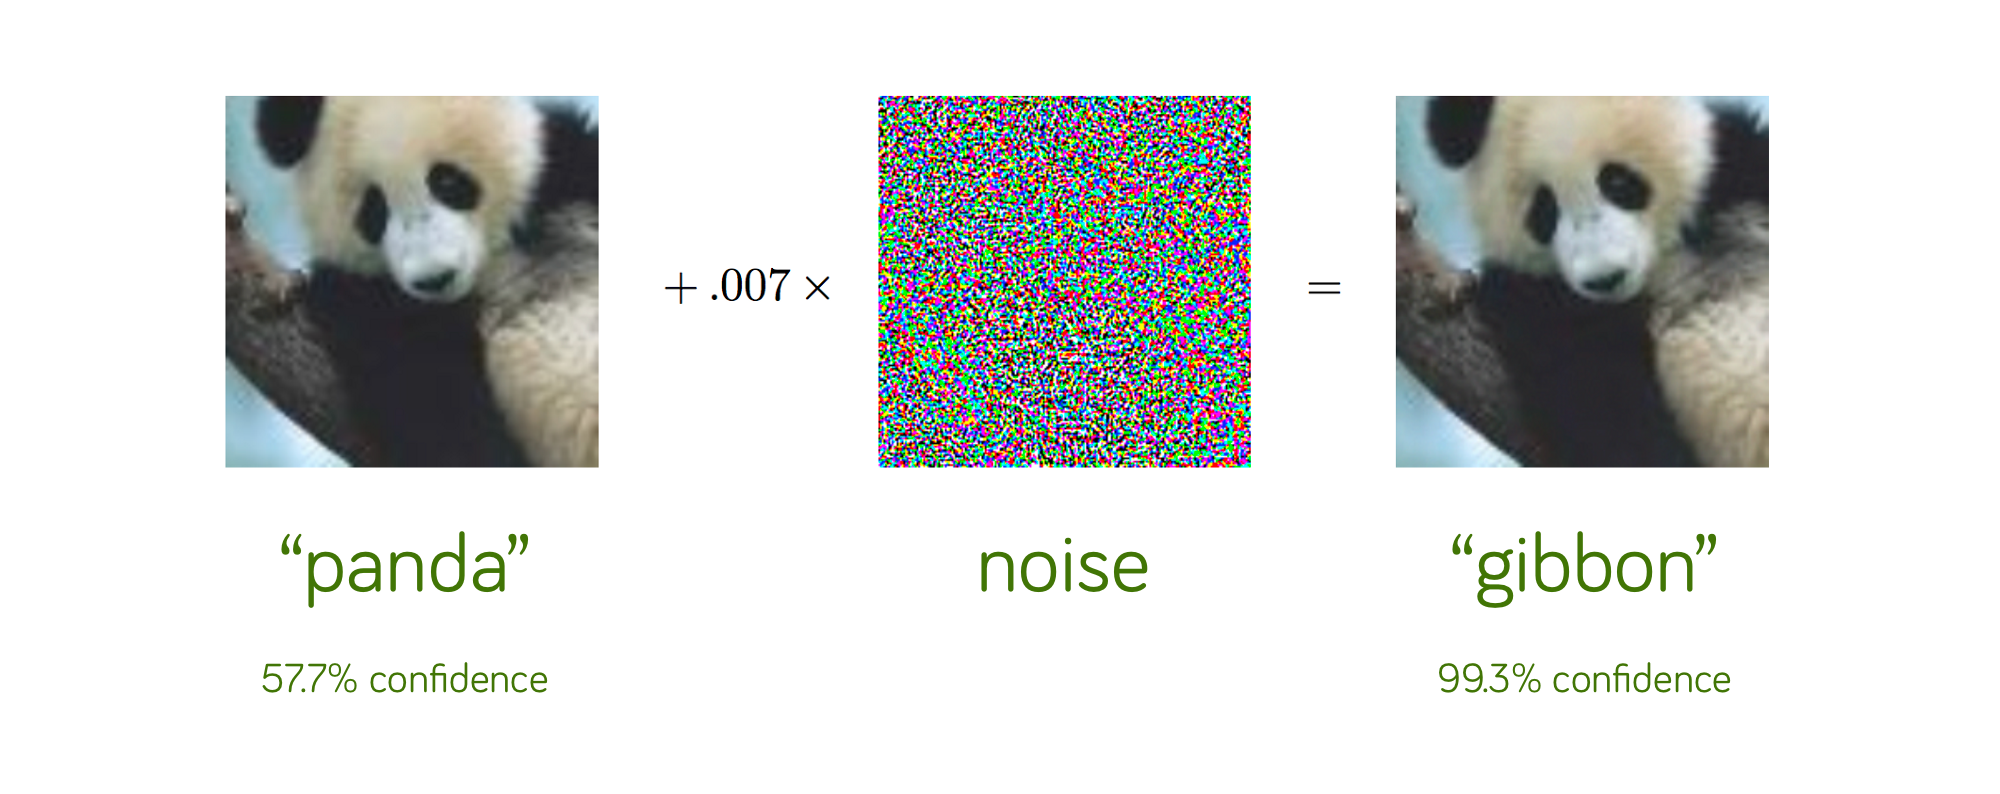
\includegraphics[scale=0.17]{attack_supervsied.png}
    \caption{Adversarial attack in classification.}
\end{figure}
\blfootnote{Goodfellow, I. J., Shlens, J., Szegedy, C. (2014). Explaining and harnessing adversarial examples.}
\end{frame}

\begin{frame}{Adversarial attacks}
"Adversarial policies: Attacking deep reinforcement learning".
\begin{itemize}
    \item It is not possible to modify the observation of an other agent.
    \item But can we attack them with adversarial observation?
    \item This is the goal of this paper: \\ How to learn to win by not directly playing the game but by performing adversarial policies.
\end{itemize}
\vfill
Framework: Zero sum Markov Game.
\vfill
Goal: black box attack by learning adversary policies.
\vfill

Examples: \href{https://adversarialpolicies.github.io/}{Website} or \href{https://www.youtube.com/watch?v=XPFQ9TBvtCE}{Video}
\end{frame}

\begin{frame}{Adversarial attacks}
How to attack a trained agent?
\begin{itemize}
    \item Victims are trained with self-play.
    \item In the paper, they take pre-trained networks between $680$ and $1360$ millions timesteps.
    \item By fixing the victim policy $\pi_\nu$, an adversarial policy $\pi_\alpha$ is trained.
    \item Note that the agent is now in a MDP since $\pi_\nu$ is now stationary.
    \item Adversarial policy is trained for $20$ millions timesteps.
\end{itemize}
\vfill
Attacks are validated by masking the position of the attacker from the victim which now wins: the attacker did not learn a strong policy.
\vfill
Fine-tuning against the attacker allows to defend against these attacks.
\end{frame}
\section{Summary}
\begin{frame}{Summary}
A non-exhaustive overview of multi-agent reinforcement learning.
\begin{itemize}
    \item Cooperative setting with partial observations:
    \begin{enumerate}
        \item QMIX
        \item COMA
        \item QVMIX
        \item Infrastructure management planning
    \end{enumerate}
    \item Communication:
    \begin{enumerate}
        \item RIAL
        \item DIAL
    \end{enumerate}
    \item Competitive setting:
    \begin{enumerate}
        \item Minimax-Q
        \item AlphaGo Zero
        \item Hide and seek
        \item Two-Team Markov Game
    \end{enumerate}
    \item Adversarial policies
\end{itemize}
\end{frame}

\begin{frame}{Additional content}

\begin{itemize}
    \item Multi-Agent Reinforcement Learning:
Foundations and Modern Approaches \url{https://www.marl-book.com/}.
\item Multi-agent RL seminars: \url{https://sites.google.com/view/berkeleymarl/home}.
\item Multi-agent learning course: \url{https://emerge-lab.github.io/multi-agent-learning/}.
\end{itemize}

    
\end{frame}

\begin{frame}[plain]{}
\center{\Huge Thank you!}
\end{frame}


\begin{frame}{References}
\begin{itemize}
    \item DQN: Mnih, V., Kavukcuoglu, K., Silver, D. et al. (2015). Human-level control through deep reinforcement learning.
    \item DRQN: Hausknecht, M., Stone, P. (2015). Deep recurrent q-learning for partially observable mdps.
    \item Markov Game and Minimax Q: Littman, M. L. (1994). Markov games as a framework for multi-agent reinforcement learning.
    \item Dec-POMDP: Oliehoek, F. A., Amato, C. (2016). A concise introduction to decentralized POMDPs.
    \item IQL: Tan, M. (1993). Multi-agent reinforcement learning: Independent vs. cooperative agents.
\end{itemize}
\end{frame}



\begin{frame}{References}
\begin{itemize}
    \item  IGM and QTRAN: Son, K., Kim, D., Kang, W.J., Hostallero, D.E. , Yi, Y.. (2019). QTRAN: Learning to Factorize with Transformation for Cooperative Multi-Agent Reinforcement Learning.
    \item VDN: Sunehag, P., Lever, G., Gruslys, A., Czarnecki, W. M., Zambaldi, V., Jaderberg, M., ...  Graepel, T. (2017). Value-decomposition networks for cooperative multi-agent learning.
    \item QMIX: Samvelyan, M., Rashid, T., De Witt, C. S., Farquhar, G., Nardelli, N., Rudner, T. G., ...  Whiteson, S. (2019). The starcraft multi-agent challenge.
    \item COMA: Foerster, J., Farquhar, G., Afouras, T., Nardelli, N.,  Whiteson, S. (2018, April). Counterfactual multi-agent policy gradients. 
    \item QVMix: Leroy, P., Ernst, D., Geurts, P., Louppe, G., Pisane, J.,  Sabatelli, M. (2020). QVMix and QVMix-Max: Extending the Deep Quality-Value Family of Algorithms to Cooperative Multi-Agent Reinforcement Learning. 
\end{itemize}
\end{frame}
\begin{frame}{References}
    \begin{itemize}
    \item RIAL and DIAL: Foerster, J. N., Assael, Y. M., De Freitas, N., Whiteson, S. (2016). Learning to communicate with deep multi-agent reinforcement learning.
    
    \item CommNet: Sukhbaatar, Sainbayar, Arthur Szlam, and Rob Fergus (2016). Learning multiagent communication with backpropagation.
    \item BiCNet: Peng, Peng et al. (2017). Multiagent Bidirectionally-Coordinated Nets: Emergence of Human-level Coordination in Learning to Play StarCraft Combat Games.
    \item IC3Net: Singh, Amanpreet, Tushar Jain, and Sainbayar Sukhbaatar (2019). Learning when to communicate at scale in multiagent cooperative and competitive tasks.
    \item TarMac: Das, Abhishek et al. (2019). TarMAC: Targeted multi-agent communication.
    \item ATOC: Jiang, Jiechuan and Zongqing Lu (2018). Learning attentional communication for multi-agent cooperation.
    \end{itemize}
\end{frame}

\begin{frame}{References}
    \begin{itemize}
    \item SchedNet: Kim, Daewoo et al. (2019). Learning to schedule communication in multi-agent reinforcement learning.
    \item GACML: Mao, Hangyu et al. (2019). Learning Agent Communication under Limited Bandwidth by Message Pruning.
    \item AlphaGo: Silver, D., Huang, A., Maddison, C. J., Guez, A., Sifre, L., Van Den Driessche, G., ... Hassabis, D. (2016). Mastering the game of Go with deep neural networks and tree search.
    \item AlphaGo Zero: Silver, D., Schrittwieser, J., Simonyan, K., Antonoglou, I., Huang, A., Guez, A., ... Hassabis, D. (2017). Mastering the game of go without human knowledge.
    \item OpenAI Five: Berner, C., Brockman, G., Chan, B., Cheung, V., ... Zhang, S. (2019). Dota 2 with large scale deep reinforcement learning. 
    \item AlphaStar: Vinyals, O., Babuschkin, I., Czarnecki, W. M., Mathieu, M., Dudzik, A., Chung, J., ... Silver, D. (2019). Grandmaster level in StarCraft II using multi-agent reinforcement learning. 
    \end{itemize}
\end{frame}

\begin{frame}{References}
    \begin{itemize}
     
     \item Capture the Flag: Jaderberg, M., Czarnecki, W. M., Dunning, I., Marris, L., Lever, G., Castaneda, A. G., ...  Graepel, T. (2019). Human-level performance in 3D multiplayer games with population-based reinforcement learning.
     \item Hide and Seek: Baker, B., Kanitscheider, I., Markov, T., Wu, Y., Powell, G., McGrew, B., Mordatch, I. (2019). Emergent tool use from multi-agent autocurricula. 
     \item Adversarial policies: Gleave, A., Dennis, M., Wild, C., Kant, N., Levine, S.,  Russell, S. (2019). Adversarial policies: Attacking deep reinforcement learning. 
     \item Perolat, J., De Vylder, B., Hennes, D., Tarassov, E., Strub, F., de Boer, V., ... \& Tuyls, K. (2022). Mastering the game of Stratego with model-free multiagent reinforcement learning. Science, 378(6623), 990-996.
     \item Leroy, P., Pisane, J., Ernst, D. (2022). Value-based CTDE Methods in Symmetric Two-team Markov Game: from Cooperation to Team Competition. In Deep Reinforcement Learning Workshop, NeurIPS.
    \end{itemize}
\end{frame}
\end{document}
    
    
    

